% Clase del documento:
\documentclass[a4paper,12pt]{article}

% Paquete geometry para establecer los márgenes:
\usepackage[inner=3.5cm, outer=3cm, top=4cm, bottom = 4cm,
            headheight=2cm, headsep=1.5cm, footskip=1.5cm]{geometry}

\usepackage[T1]{fontenc}
\usepackage[utf8]{inputenc}
\usepackage[spanish,es-tabla]{babel}

% Paquete para imprimir codigo:
\usepackage{listings}
% Paquetes para imprimir pseudocodigo:
\usepackage{algorithm} 
\usepackage{algpseudocode}
% traducción
\floatname{algorithm}{Algoritmo}
% Paquetes para ecuaciones y numeros:
\usepackage{amsmath}
%Para las tabla y colores
\usepackage[table]{xcolor}
\usepackage{array}
\usepackage{hhline}

\usepackage{nicematrix}


% Paquete para espaciado e interlineados:
\usepackage{setspace}

% Paquete para incluir figuras y gráficos:
\usepackage{graphicx}

\usepackage{titlesec}
\usepackage{appendix}

% Estilo de enlaces y urls:
%\usepackage[usenames]{color}
\usepackage{hyperref}
\usepackage{url}

\hypersetup{
    colorlinks=true,
    linkcolor=black,
    urlcolor=blue,
%    citecolor=blue
}

% Estilo de paginas:
\usepackage{lmodern}
\usepackage{fancyhdr}

\usepackage{etoolbox}
\patchcmd{\thebibliography}{\section*{\refname}}{}{}{}
%%%%%%%%%%%%%%%%%%%%%%%%%%%%%%%%%%%%%%%%%%%%%%%%%%%%%%%%%%%%%%%%%%%%%%%%%%%%%%%

\title{{\Large{Trabajo de Fin de Grado}} \\
        \vspace{1.25cm}
        {{\textbf{Evaluación de Prestaciones de Rutinas Matriciales Paralelizadas con Intel oneAPI en \\ Sistemas Heterogéneos}}}  \\
        \vspace{1cm}
        \begin{figure}[htbp]
            \centering
	        
\includegraphics[scale=0.25]{./images/logo-um.png}
        \end{figure}
}
\author{\Large{Universidad de Murcia} \\
        \\
        \\
        Autor:
        \\
        \large{Miguel Ángel Rodríguez García} \\
        \\
        \\
        Directores:
        \\
        \large{Javier Cuenca y José Matías}
        \\
        \\
}
\date{\Large{2025}}
%%%%%%%%%%%%%%%%%%%%%%%%%%%%%%%%%%%%%%%%%%%%%%%%%%%%%%%%%%%%%%%%%%%%%%%%%%%%%%%

% Comienzo del documento:
\begin{document}

% Se establece el interlineado del documento:
%\onehalfspacing

% Se establece la separación entre párrafos:
\setlength{\parskip}{0.15cm}

% Se crea la portada:
\maketitle
\thispagestyle{empty}


\newpage

\null\cleardoublepage

\newpage

%%%%%%%%%%%%%%%%%%%%%%%%%%%%%%%%%%%%%%%%%%%%%%%%%%%%%%%%%%%%%%%%%%%%%%%%%%%%%%%
\section*{Resumen}
%%%%%%%%%%%%%%%%%%%%%%%%%%%%%%%%%%%%%%%%%%%%%%%%%%%%%%%%%%%%%%%%%%%%%%%%%%%%%%%

Este trabajo trata sobre nuevas herramientas que se utilizan en la computación paralela. Dicha computación consiste en distribuir las tareas de un algoritmo entre los distintos elementos de procesamiento. Estos elementos pueden ser nodos de clusters, CPU's o procesadores en el caso de programación mediante paso de mensajes (memoria distribuida) o simplemente procesadores o hilos en el caso de la computación paralela mediante memoria compartida. De forma que, hoy en día, gracias a los avances tecnológicos acaecidos en los últimos años, se consiguen resolver problemas que antes no se podían resolver con un solo elemento de procesamiento, ya que no se tenían recursos suficientes. La computación paralela tiene gran relevancia en muchas áreas hoy en día, como puede ser en aplicaciones relacionadas con la astronomía, con la predicción climática, con el cálculo de constantes y funciones numéricas, etc.

Las herramientas sobre las que se va a realizar un análisis son las dos librerías nuevas que ha desarrollado Intel orientadas a la programación paralela. Estas librerías son Intel MPI Library, orientada a usarse en memoria distribuida (paso con mensajes), e Intel oneAPI Threading Building Block (OneTBB), orientada a usarse en memoria compartida. Además de estudiar estas dos librerías por separado, se van a estudiar también de forma conjunta, es decir, se implementa un código híbrido que usa las dos librerías a la vez.

Para este estudio se han utilizado como referencia dos de las librerías de código abierto más usadas hoy en día en la programación paralela, como son Open MPI, usada en memoria distribuida, y OpenMP, usada en memoria compartida. Al igual que con las librerías de Intel, se realizará una implementación híbrida en la que se usarán estas dos librerías de forma conjunta para poder comparar los resultados obtenidos con el híbrido de Intel.

El método de comparación entre las nuevas librerías de Intel y las de Open es mediante el uso de ellas en la implementación de un programa donde se realiza la rutina multiplicación de matrices por bloque (MMB). Esta rutina es elegida debido a que gran parte de su código se puede paralelizar, y también, a que puede escalar fácilmente simplemente aumentando el tamaño del problema (tamaño de las matrices).

En este estudio tendremos seis implementaciones distintas de la rutina MMB, y dichas implementaciones se comparan de dos en dos. Primero compararemos las implementaciones que usan librerías de memoria compartida, es decir, OpenMP con Intel TBB. Luego, las que usan librerías de memoria distribuida, Open MPI con Intel MPI. Finalmente, compararemos la implementación del híbrido OpenMP-Open MPI con el del híbrido Intel TBB-Intel MPI.

La paralelización de estas seis implementaciones ha sido de grano grueso, es decir, hemos paralelizado los primeros dos bucles donde en su interior se desarrolla la multiplicación de matrices por bloque, de forma que las comunicaciones entre los hilos/procesos han sido las menos posibles. En memoria compartida, se ha conseguido paralelizando los bucles exteriores, en el caso de OpenMP usando al principio de los bucles de la rutina {\it MMB} la directiva {\it parallel for} junto a la directiva {\it collapse}, haciendo que los dos bucles se hagan como solo uno y repartiendo el trabajo que hay en los dos entre los hilos. En cuanto a Intel TBB, se ha aplicado la misma idea pero con otro método que tienen para ello, esta función se llama {\it blocked\_range2d}, que básicamente hace lo mismo que en OpenMP, reparte el trabajo que hay en los dos bucles sobre los hilos existentes.

En cuanto a las implementaciones de Open MPI e Intel MPI, han sido las mismas, debido a que aunque las librerías trabajan de forma diferente internamente, por fuera sus funciones tienen los mismos nombres, haciendo que los códigos de las dos versiones sean idénticos. Por ello, en la implementación de estas dos librerías se ha utilizado la llamada {\it MPI\_Bcast} para el reparto de la matriz B, pues se necesita en todas, y luego la llamada {\it MPI\_Scatter}, para repartir las filas de la matriz A con las que realizará sus multiplicaciones de bloques cada proceso. Después, cada proceso hará el secuencial de la rutina {\it MMB} obteniendo así sus filas de la matriz resultado. Por último, cada proceso llamará a {\it MPI\_Gather} entregando estas filas calculadas al proceso 0.

Las últimas implementaciones realizadas fueron las de los híbridos de Open e Intel. Éstas se hicieron con la mezcla de las dos anteriores, es decir, para el híbrido de Open se usaron las llamadas a {\it MPI\_Bcast} y {\it MPI\_Scatter} para repartir el trabajo en memoria distribuida entre los procesos, y luego en el secuencial de la rutina MMB, este utiliza las directivas que se usan en OpenMP, haciendo que ya no sea secuencial y, por tanto, paralelizando también la rutina. Por último, una vez los procesos ya obtienen sus filas de la matriz resultado lo juntan de nuevo mediante {\it MPI\_Gather}. En el híbrido de Intel se siguen los mismos pasos, pero en vez de usar las directivas de OpenMP se han usado los métodos que hemos mencionado de Intel TBB.

Las comparaciones se han basado en los tiempos de ejecución que han obtenido las seis implementaciones, la ejecución de estos seis códigos se ha realizado en el nodo Venus del clúster de la Facultad de Informática de la Universidad de Murcia, cuyas prestaciones a destacar son que tiene 2 CPU's Intel Xeon E5-2620 (hexa-core) que funcionan a una frecuencia de 2.40 GHz y tienen una arquitectura x86-64. Dispone de una arquitectura de memoria tipo NUMA con 64 GB de memoria RAM, caches L1 y L2 privadas por core de 32 KB y 256 KB, respectivamente, y una caché L3 de 15 MB compartida por todos los cores de cada socket (NUMA-Node).

Para la ejecución de estas seis implementaciones en el nodo Venus primero se ha estudiado el tamaño de submatriz (bloque) que sería utilizado en la comparación de este estudio. Esto se debe a que el tamaño de las submatrices influye en los tiempos de ejecución, debido a que cuando traemos un número de una matriz, también traemos los números contiguos aprovechando la localidad espacial (se trae la página de datos entera a la caché), es decir, traemos la fila (entera o parcial) de la matriz donde está ese número. Esta investigación, en teoría demostraba que el tamaño de submatriz correcto para las características del nodo Venus debería haber sido de 32$\times$32, pero en la práctica se ha visto que el tamaño correcto era el de 16$\times$16, esto era debido a que nosotros teóricamente suponíamos que solo las submatrices usadas en la multiplicación por bloque estarían en caché, pero es muy posible que otros datos también estuvieran en caché haciendo que en la práctica el bloque ideal fuera más pequeño, en este caso 16$\times$16. Este tema ha sido interesante porque se ha visto cómo influyen los aciertos y fallos de la caché en los tiempos de ejecución, pero no se ha profundizado más, simplemente se ha sacado el bloque de submatriz óptimo que utilizaremos en nuestro estudio principal.

A continuación, se ha procedido a ejecutar y comparar los tiempos de ejecución, primero de los programas paralelos que usaban las librerías OpenMP e Intel TBB, las que están orientadas a memoria compartida. En esta primera comparación, se ha comprobado que, cuanto más grande era el tamaño del problema y se tenía un mayor número de hilos, Intel TBB obtiene mejores resultados que OpenMP, llegando aproximadamente a haber hasta un 115\% de diferencia en los {\it speed-up} (respecto al secuencial) de las dos dos implementaciones a favor de IntelTBB en el mejor de los casos.

En cuanto a los tiempos que se obtienen para las librerías orientadas a memoria distribuida, Open MPI e Intel MPI, éstos son muy parejos, siendo incluso algo mejor los de Open MPI cuando el tamaño del problema no es muy grande y no hay muchos procesos. En cambio, los tiempos de Intel MPI que destacan sobre Open MPI son cuando se utiliza un número mayor de procesos y el tamaño del problema es más grande. Los speed-up en estas configuraciones han sido muy parejos, variando las diferencia de {\it speed-up} entre un 93\% aproximadamente en la peor configuración para Intel MPI hasta un 104\% en la mejor comparación.

En la última comparación de tiempos de ejecución, esta vez entre los híbridos de Open y los híbridos de Intel, el híbrido de Intel ha destacado sobre el de Open. Esto es debido a que se ha acercado mucho a los tiempos que se han dado en memoria distribuida (mejores tiempos que en memoria compartida). En cambio el híbrido de Open ha empeorado, haciendo que el híbrido de Intel obtenga mejor {\it speed-up} que el híbrido de open con cualquier configuración, cosa que no había ocurrido en las comparaciones anteriores, esta diferencia entre los {\it speed-up} ha sido de hasta un 125\% a favor del híbrido de Intel.

Una vez sacado los tiempos de ejecución y hecho las comparaciones entre las distintas implementaciones, hemos explicado el por qué de estas diferencias de tiempo entre las distintas librerías. Para ello, hemos utilizado otra herramienta de Intel con la que podemos analizar los códigos de muchas otras formas. Esta herramienta se llama {\it profiling Intel VTune}. En concreto, dentro de esta herramienta hemos utilizado el método de análisis llamado {\it threading}, con el que podemos ver lo bien estamos paralelizando el código. Esto se ve gracias a que la herramienta, entre otras cosas, nos muestra los tiempos que transcurren en cada función, el porcentaje y el uso de la CPU, el tiempo de ejecución paralelo, etc.

Finalmente, podemos concluir que para nuestros entornos usados y la rutina MMB, las librerías Intel TBB e Intel MPI obtienen mejores resultados que dos de las librerías de programación paralela más usadas hoy en día, como son OpenMP y Open MPI. Este resultado, como hemos dicho, se da para nuestro entorno y para la rutina {\it MMB} que hemos creado. Con esta idea en mente, queda como trabajo futuro realizar más comparaciones entre estas librerías con otras rutinas y entornos, de forma que puedan aportar otras conclusiones y se complemente el trabajo realizado.




\newpage

%%%%%%%%%%%%%%%%%%%%%%%%%%%%%%%%%%%%%%%%%%%%%%%%%%%%%%%%%%%%%%%%%%%%%%%%%%%%%%%
\section*{Extended Abstract} % In English (extensión Mínima: 2000 palabras)
%%%%%%%%%%%%%%%%%%%%%%%%%%%%%%%%%%%%%%%%%%%%%%%%%%%%%%%%%%%%%%%%%%%%%%%%%%%%%%%
\thispagestyle{empty}
This paper deals with the new tools used in parallel computation. Said information technology consists of distributing the tasks of an algorithm between the different elements of processing. These elements can be cluster nodes, CPU’s or processors in case of  programming by message exchange (distributed memory) or just processors or threads in case of parallel computation by shared memory in order to resolve the problems that could not be solved before with just one element of processing because of the insufficient resources. This parallel computation has huge relevance in multiple areas today, like astronomy related applications, climatic prediction, constant calculations and numeric functions, etc.




The tools the analysis is going to be over, are the two computer libraries designed by Intel aimed at parallel programming. These are Intel MPI Library, focused on distributed memory, and Intel oneAPI Threading Building Block (OneTBB), focused on Shared memory. Besides studying these libraries separately, they are going to be studied together, that is to say a hybrid code is introduced and it uses both libraries at the same time.

For this study two of the most used open source libraries used for parallel programming are going to be used as reference, these are Open MPI, for distributed memory, and Open Mpi, for shared memory. As in Intel libraries, a hybrid implementation is going to be used in order to use both libraries at the same time to compare the Intel Hybrid.

The comparative method between the new Intel libraries and the aforesaid of Open is by their use in the implementation of a program where it does the block matrix multiplication (BMM). This routine is selected because a great part of its code can be done alongside and also because it can move up just by increasing the size of the problem (size of the matrix).

Said that, in this study we will have six different implementations of the BMM routine, and these implementations are compared two by two. First, we will compare the ones that use shared memory libraries, OpenMP with Intel TBB. Then, the ones that use distributed memory libraries, Open MPI and Intel MPI. Finally, we will compare the implementation of the hybrid OpenMP-OpenMPI, with the hybrid Intel TBB-Intel MPI.

The parallelization of these six implementations are (whole grain), that is, we have parallelized the outside part of the sequential of the block matrix multiplication. In the way that the communications between the threads/processes are the least possible. In shared memory we have achieved it by parallelising the outside loop, in the case of OpenMP, using at the beginning of the loops of the BMM routine the directive parallel with the directive collapse (2), making that the two loops become one and divide the work between the threads. Regarding Intel TBB, it has been applied the same idea but with another method, this function is called blocked\_range2d and basically it does the same as in OpenMP, divides the work of the loops between the existent threads.

Regarding the implementations of OpenMPI and IntelMPI, they have been the same, because even though the libraries work in different ways internally, on the outside its functions have the same names, making the code of the two versions identical. Because of that, for the implementation of these two libraries we have used MPI\_Bcast to distribute the B matrix, and then, MPI\_Scatter to distribute the lines of the A matrix with which each process will do its block multiplications. Later, each process will do the secuencial of the BMM routine, achieving that way its result matrix lines and, at last, each process will call MPI\_Gather, giving that lines calculated at 0 process.

The last implementations have been the ones of the hybrids of Open and Intel. They have been made with the mix of the two implementation said before, it is, for the hybrid of Open we make the calls to MPI\_Bcast and MPI\_Scatter to divide the work in distributed memory between the processes, and then, in the sequential of the routine BMM it is used the directives used in OpenMP, stopping it from being sequential and parallelizing the routine. At last, once the processes obtain their result matrix lines it is put together again by MPI\_Gather. In the Intel hybrid the same steps are followed, but instead of using the directives of OpenMP we used the methods already mentioned by Intel TBB.

These comparatives are based on the execution times made by the six implementations and  taking as a reference the execution time of the sequential version of the BMM routine. Its execution has been done in the Venus node of the computing department of the University of Murcia cluster, whose destacable features are two Intel Xeon E5.2620 (hexa-core) CPU’s that work at 2,40 GHz and have a x86-64 architecture. It has a NUMA type memory architecture with 64GB RAM, private L1 and L2 cache per core of 32KB and 256KB, respectively, and a L3 cache of 15MB shared by every core of each socket (NUMA-Node).

For the execution of the six implementations in the Venus node, first we have studied the size of the submatrix that would be used for the comparison of this study. This is because the size of the submatrix affects the execution times. When we take a number from a matrix, we also take the adjacent numbers, taking advantage of the spatial location (the full data page is brought to the cache), that is, we bring the line (whole or partially) from the matrix where that number is. This research, in theory, demonstrates that the correct submatrix size for the Venus node characteristics should have been 32$\times$32, but in practice it has been seen that the correct size is 16$\times$16, this is due that theoretically we supposed that just the submatix used in the block multiplication would be in the cache, but it is very likely that other data were also in the cache, for this, in practice the ideal block is smaller, in this case 16$\times$16. This topic has been very interesting because we see how the right and wrong answers of the cache affect the execution times, but it has not been studied in more detail, we just brought the ideal submatrix block that we are going to use in our main study.

After that, we have executed and compared the execution times, first the ones of the parallel programs that use OpenMP and Intel TBB, focused on shared memory. In this first comparison it has been seen that with bigger problem size and more number of threads, Intel TBB is better than OpenMP, 115\% better in the best cases. This number has been calculated by dividing the speed-up (regarding the sequential code) between the two versions.

Regarding the times seen for the distributed memory libraries, Open MPI and Intel MPI are very similar, being almost better than the Open MPI ones when the size of the problem is not very big and there are not many processes. On the other hand the times of MPI stand out above MPI when a bigger number of processes are used and the size of the problem is bigger. Being a 93\% superior in the worst of cases and up to a 104\% in the better of the comparisons.

In the last comparison of execution times, this time between the hybrinds of Open and the Hybrids of Intel, the Intel Hybrid stands out. This is because the time of distributed memory has been very similar (better times than in shared memory), but the Open hybrid has been left behind, having the Intel hybrid an advantage of a 125\% in the best cases, and having better times with every configuration, what did not happen in previous comparisons

Once the times have been noted and the comparisons done between the implementations, we are going to explain why there is such a time difference between the libraries. For this, we have used an Intel tool named profiling Intel VTune, which lets us analyse the codes in multiple ways. From this tool we have used the analysis method called threading, with whom we can see how well parallelized the code is. This is thanks to that the tool, among other things, shows us the times of each function, the percentage of use of the CPU, the time of parallel execution, etc.

Going back to the comparisons between OpenMP and Intel TBB, the tool Intel VTune, shows us that Intel TBB takes a few tenths more than OpenMP in the creation of threads and the later work between them. But it also shows us that in OpenMP the time that passes in the call where the submatrix multiply is bigger than in intel TBB. This is because, after a deeper study of Intel TBB we have found that it does not assign its threads the work at once, like OpenMP, but it asign a little quantity of work making possible that its threads be able to work in close memory regions, making it possible to have right answers in cache thanks to the spatial location. However, OpenMP assigns the work all at once so the threads work in far areas and it lowers the right answers in cache because they do not use the spatial location. Thus, even if Intel TBB at first spends more time in the assignment of work, it eventually achieves better times than OpenMP because of said reason.

In the comparison between OpenMP and Intel MPI, the tool VTune has shown us the reason why the times, although similar, the ones of Intel MPI are a little better than the ones of Open MPI when the size of problem is bigger. We have seen that the times of the functions that communicate with the processes, that are MPI\_Bcast, MPI\_Scather, MPI\_Gather, are a little slower in Open MPI than in Intel MPI. Being this the reason why Intel MPI has better times than Open MPI, specially when the problem is bigger, because those functions take more time and make visible the difference between Intel MPI and OpenMP.

Finally, with Intel VTune we have analysed the comparisons between the hybrids of Open and Intel. This leads to the vision of the differences already mentioned  in the previous comparisons when they have been implemented alone. Furthermore, the times have shoot up in the function mentioned in shared memory, this function where the matrix multiply, is now executed slower than before, and also the calls to the functions of MPI are a little slower in the Open Hybrid, whereas the Intel Hybrid the times are very similar to the ones shown before, this makes us believe than the Intel hybrid coordinates better the use of both its libraries Intel TBB and Intel MPI. On the other hand, Open coordinates worse than Intel the mix of its libraries and makes its times higher, as seen before.

We can conclude that for our used surroundings and the BMM routine, the Intel TBB and Intel MPI libraries give better results than two of the more used libraries of parallel programming, which are OpenMP and Open MPI. This result, as we have said before, is for our surroundings and the BMM routine; with this idea in mind, we have as a future work, carry out more comparisons between these libraries with other routines and surroundings, in a way that work can provide further conclusions and complement this study.

The main objective of this study was making a comparison between the OpenMP and IntelTBB libraries of shared memory, Open MPI and IntelMPI libraries of distributed memory and between the hybrids of Open and Intel. The analysis of all these comparatios has been made focusing mainly on the times of execution that each implementation has given and, thanks to the use of the tool Intel VTune we have been able to explain the reason of the different times of execution and, that way, make a comparison and a further analysis between the different libraries of Open and Intel, concluding that intel TBB and Intel MPI libraries give better results than two of the most used parallel programming libraries today, that are OpenMP and Open MPI.

This result, as we have said, occurs in the computing environment we have worked in and in the BMM routine. For this, even when we have obtained advanced conclusions about these libraries thanks to the comparisons made, they are not definitive, because other comparisons may be done and different analysis with different points of view. It is left for future research, comparisons with other routines like establishing a different focus than the loops and the parallelization of tasks or lowering the relevance of the right and wrong answers in cache. For distributed memory we could, for example, make a routine were other calls, different ones to the ones we have used, take the prominence, to see if we obtain the same results or a finer grain routine where more communications between processes has to be made, to see if the advantage of Intel MPI becomes more representative.

\newpage

\tableofcontents
\thispagestyle{empty}

\newpage

%%%%%%%%%%%%%%%%%%%%%%%%%%%%%%%%%%%%%%%%%%%%%%%%%%%%%%%%%%%%%%%%%%%%%%%%%%%%%%%
\section{Introducción} \label{sec:introduccion}
%%%%%%%%%%%%%%%%%%%%%%%%%%%%%%%%%%%%%%%%%%%%%%%%%%%%%%%%%%%%%%%%%%%%%%%%%%%%%%%

Inicialmente, en la programación, los códigos se escribían para ejecutarse de forma secuencial, es decir, las instrucciones se ejecutaban una detrás de otra en el procesador principal, de forma que hasta que no terminaba completamente la ejecución de una, no se podía ejecutar la siguiente instrucción. Mediante esta idea se creaban programas estructurados y fáciles de comprender, pero tenían el inconveniente de que eran lentos, ya que desaprovechaban gran parte del {\it hardware}.

Con el paso del tiempo surgió la necesidad de resolver problemas cada vez más grandes y complejos, pero con la configuración anterior de ejecución de instrucciones esta tarea se hacía realmente complicada. Entonces surgió la idea de aumentar la rapidez de la ejecución de estas instrucciones en el procesador aumentando el número de transistores dentro de cada procesador, de tal forma que se aumentó la frecuencia y disminuyó el tiempo de ejecución final. En este sentido, el cofundador de Intel, Gordon E. Moore, enunció en el año 1965 lo que a posteriori se conoció como la ley de Moore~\cite{LeyMoore}, en la que se establecía que el número de transistores en un microprocesador se duplicaría aproximadamente cada dos años.

Ha llegado un momento en que esta mejora del {\it hardware}, en cuanto a mejora computacional, está llegando a un límite debido a que un aumento en la frecuencia aumenta la cantidad de energía utilizada en un procesador, tal y como podemos ver en la Figura~\ref{fig:moore}. El estancamiento de la Ley de Moore es una consecuencia del límite físico de la tecnología actual. Al aumentar la densidad de transistores también se aumenta el calor generado para un mismo volumen. Por lo tanto, no es posible extraer el calor suficientemente rápido sin riesgo a sobrecalentar y dañar el microprocesador. Además, normalmente los transistores se hacen cada vez más pequeños para aumentar la cantidad de éstos en los chips, sin cambiar el tamaño de estos últimos, lo cual tiene un límite físico impuesto por el tamaño de los átomos. Aunque se han propuesto soluciones para poder seguir aumentando el rendimiento de los procesadores manteniendo un tamaño razonable.

\begin{figure}[htbp]
    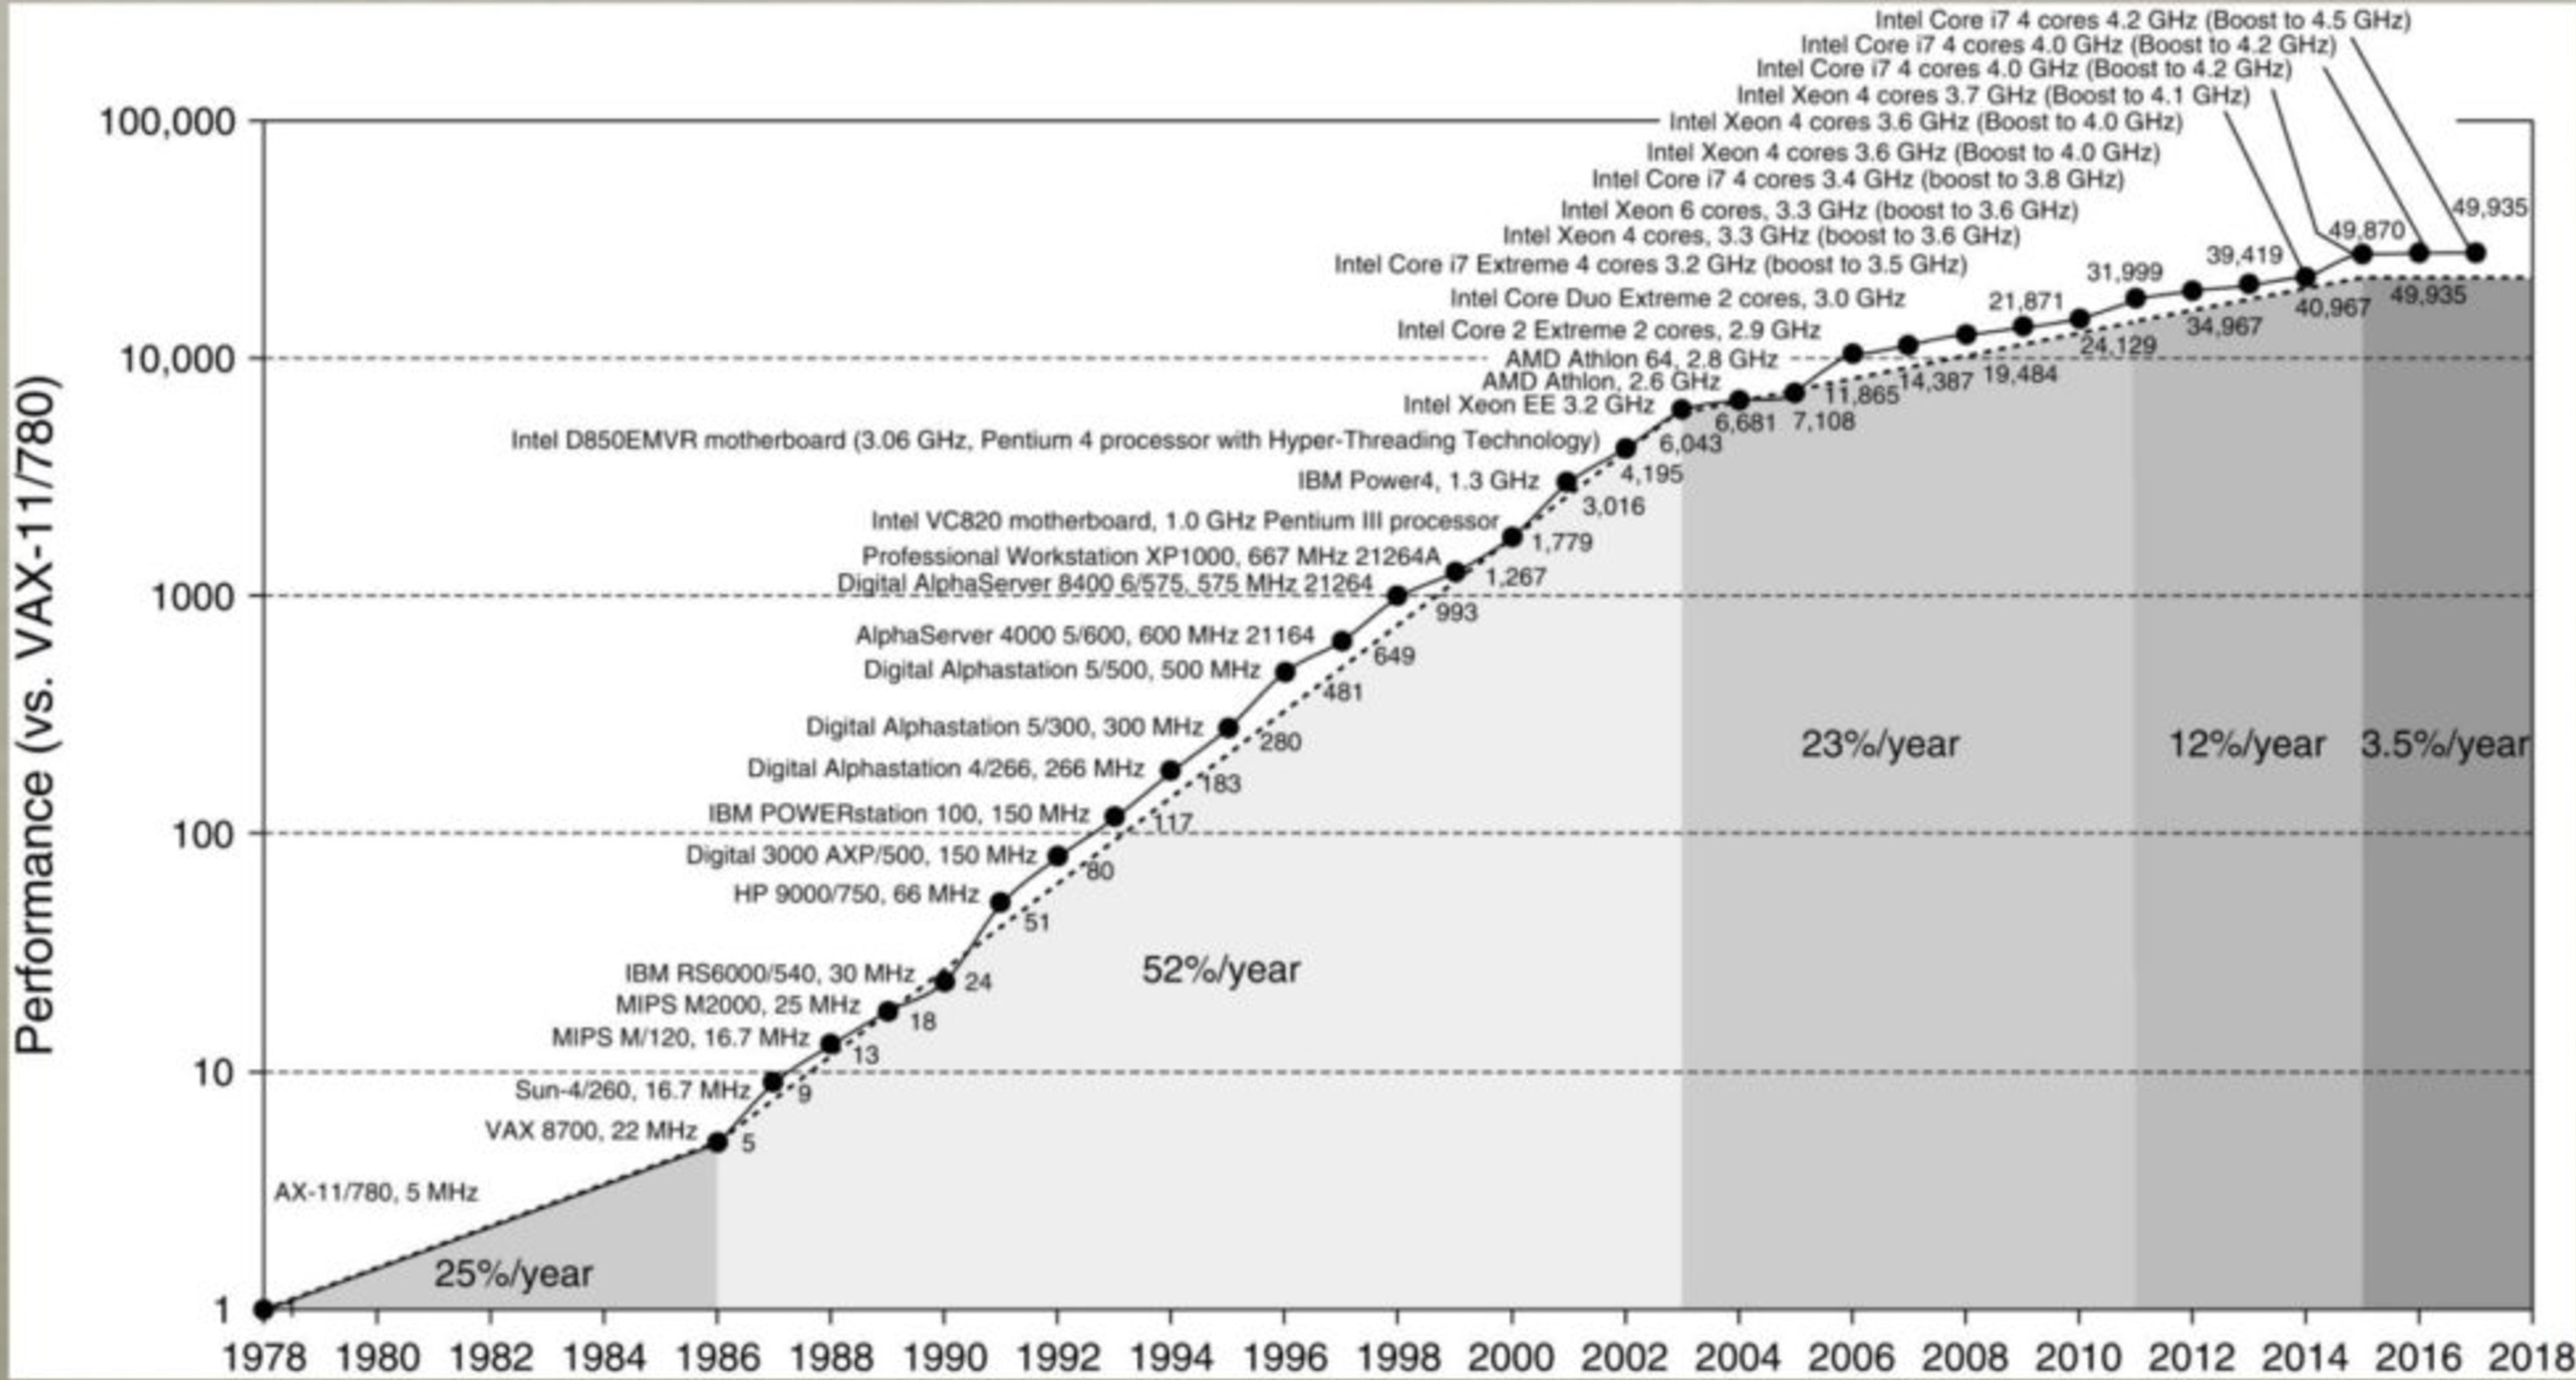
\includegraphics[width=1\textwidth]{./images/leymoore.pdf}
    \centering
    \caption{Evolución gráfica de la ley de Moore~\cite{endMoore}.}
    \label{fig:moore}
\end{figure}

Este aumento del consumo de energía del procesador llevó a Intel, en mayo del 2004, a la cancelación de dos de sus procesadores en desarrollo. Este hecho generalmente es conocido como el fin del escalado de frecuencia como el paradigma dominante de arquitectura de computadores.

Debido a esto, se comenzaron a explorar otras formas de seguir acelerando la ejecución de los programas, y una de ellas fue la computación paralela. La técnica se basa en el principio, según el cual, algunas tareas se pueden dividir en partes más pequeñas que pueden ser resueltas simultáneamente. Dicha computación consiste en poder ejecutar en tiempo de ejecución varias instrucciones a la vez repartidas en distintos elementos de procesamiento. Estos elementos de procesamiento son variados e incluyen recursos tales como una CPU con múltiples núcleos, varios ordenadores en red conectados entre sí, hardware especializado, o cualquier combinación de los anteriores. En nuestro caso hemos utilizado el primero, una CPU (ordenador del alumno) y varios nodos de cluster (proporcionado por la universidad) con múltiples procesadores.

Aunque el paralelismo también tiene sus propias restricciones, estas vienen marcada por la ley de Amdahl~\cite{Amdahl}. Esta ley establece que ``{\it La mejora obtenida en el rendimiento de un sistema debido a la alteración de uno de sus componentes está limitada por la fracción de tiempo que se utiliza dicho componente}''. Es decir, la proporción de mejora que se recibe en la ejecución de un programa por el paralelismo va relacionada con la fracción de código que esta se puede paralizar, pues en general, un programa nunca es 100~\% paralelizable. Entre esta restricción y que para aplicarlo correctamente se necesitan unos amplios conocimientos y un gran esfuerzo, es por ello, que el paralelismo es una gran herramienta que se puede utilizar en determinadas ocasiones y grandes problemas de cálculo, pero no predomina en el mundo de la programación.

Actualmente, en la programación paralela, se suele trabajar con dos librerías/estándares, de código abierto, como son OpenMP~\cite{openmp} (en memoria compartida, multihilo) y  Open MPI~\cite{openmpi} (con paso de mensajes, multiprocesador), además de un método híbrido que mezcla las dos librerías anteriores.

Llegados a este punto, vamos a realizar un estudio para ver si las nuevas herramientas de paralización de Intel llamadas {\it Intel MPI Library}~\cite{impi} e {\it Intel oneAPI Threading Building Blocks (OneTBB)}~\cite{tbb} ofrecen mejores prestaciones que las tradicionales.

\newpage
%%%%%%%%%%%%%%%%%%%%%%%%%%%%%%%%%%%%%%%%%%%%%%%%%%%%%%%%%%%%%%%%%%%%%%%%%%%%%%%
\section{Estado del Arte} \label{sec:estado_arte}

%%%%%%%%%%%%%%%%%%%%%%%%%%%%%%%%%%%%%%%%%%%%%%%%%%%%%%%%%%%%%%%%%%%%%%%%%%%%%%%
En esta sección vamos a hablar del estado actual de las diferentes librerías, así como de los principales casos de uso que tienen y sus aplicaciones.

\subsection{Estado actual y usos de las librerías OpenMP y Open MPI}

Open MPI y OpenMP son dos de los principales modelos de programación que se han utilizado ampliamente durante muchos años para la computación de alto rendimiento. Se han realizado numerosos esfuerzos para estudiar diversos aspectos de los dos modelos, desde la programabilidad hasta el rendimiento, usándose en la actualidad para la mejora del rendimiento en numerosas herramientas.

En la página oficial de la librería de OpenMP~\cite{who} podemos encontrar un apartado con algunos ejemplos de aplicaciones que utilizan esta librería. Una de estas sería, por ejemplo, {\it MACROS}~\cite{macros}, que se declara como una ``una aplicación comercial para la automatización de procesos, el modelado predictivo, el análisis de datos intelectuales y la optimización''. Esta aplicación, además, indica que ha usado OpenMP desde el primer día de su desarrollo para mejorar el rendimiento de la herramienta.

%https://www.datadvance.net/

Otra aplicación que nos mencionan es {\it Altair RADIOS}~\cite{altair}, un entorno que se dedica a predecir con precisión los efectos dinámicos de carga transitoria en estructuras y productos para mejorar la seguridad, la capacidad de supervivencia y diseñar productos más robustos para diversas industrias, como pueden ser la automotriz, la aeroespacial y la electrónica. Esta herramienta usa un modelo híbrido de Open MPI junto OpenMP, siendo MPI el que gestiona el primer nivel de paralelización mediante comunicaciones entre los distintos nodos, y luego OpenMP, que se utiliza en el segundo nivel para mejorar el rendimiento implementando paralelismo dentro de cada nodo.

%https://www.altair.com/radioss

Otro ejemplo de uso de la librería OpenMP es el sistema de simulación astrofísica general {\it GenASiS}~\cite{genasis}. GenASiS es un código nuevo que se está desarrollando inicialmente y principalmente para la simulación de supernovas de colapso del núcleo en las supercomputadoras de mayor capacidad del mundo. GenASiS está diseñado para modularidad y extensibilidad de la física. Escrito en Modern Fortran (Fortran 2003 y 2008) y diseñado con un paradigma orientado a objetos, GenASiS todavía se encuentra actualmente en un fuerte desarrollo.

En el campo de la ingeniería hidráulica también podemos ver ejemplos de uso de la librería OpenMP. Este es el caso del modelo comercial {\it RiverFLO-2D}~\cite{riverflo2d}. RiverFLO-2D es un modelo comercial de ingeniería hidráulica bidimensional que resuelve ecuaciones de aguas poco profundas promediadas en profundidad con el método de elementos finitos. El modelo utiliza mallas de elementos triangulares que pueden tener varios cientos de miles de elementos y un esquema de integración de tiempo explícito que restringe el paso de tiempo, lo que resulta en un esfuerzo computacional considerable para simulaciones variables en el tiempo. El código está escrito en Fortran 95 y el ejecutable se genera con el compilador Intel Fortran. Para mejorar el rendimiento del modelo, hace un uso extensivo de OpenMP para paralelizar los bucles de elementos principales en plataformas de múltiples núcleos~\cite{who}.

%https://www.openmp.org/about/whos-using-openmp/

Open MPI también es usado en supercomputadoras TOP500 como la {\it Roadrunner}~\cite{super1} y la {\it K computer}~\cite{super2}, dos de las supercomputadoras más rápidas del mundo entre los años 2008 y 2012. Debido a la potencia de cálculo que ofrecía MPI al supercomputador Roadrunner, este tenía como uso principal el trabajar con armas nucleares, como la simulación de ataques nucleares. Pero, también se usa en simular interacciones complejas en muchos sectores debido a su alto nivel de procesamiento como superordenador, entre otros la medición de la desintegración nuclear, el estudio de patrones meteorológicos complejos y el desarrollo de proyecciones del mercado de capitales o cálculos astronómicos.

%https://www.techtarget.com/searchdatacenter/definition/IBM-Roadrunner

%https://www.open-mpi.org/papers/kcomputer-2012/mpi-library-and-low-level-communication-on-k.pdf


\subsection{Estado actual y usos de las librerías paralelas de Intel}

Intel TBB e Intel MPI son dos librerías novedosas y que aún continúan en desarrollo. Es por ello que no son ampliamente utilizadas, ya que en la actualidad se siguen haciendo estudios sobre cómo evolucionan y las ventajas que nos pueden ofrecer.

Intel TBB destaca en su página principal~\cite{tbb} algunos de sus usos, como que es ideal para el software que se dedica a los campos en los que se necesita un cálculo intensivo. Algunos de estos campos serían la predicción meteorológica numérica, la oceanografía, la astrofísica, la ingeniería genética, la IA y la automatización. Dos herramientas que siguen desarrollándose y usan Intel TBB son {\it MOOSE}~\cite{moose} y {\it MADNESS}~\cite{madness}. La primera trabaja sobre un entorno de simulación orientado a objetos de multifísica, mientras que la segunda proporciona un entorno de alto nivel para la solución de ecuaciones integrales y diferenciales en muchas dimensiones utilizando métodos adaptativos y rápidos.

%1.https://github.com/idaholab/moose

%2.https://github.com/m-a-d-n-e-s-s/madness

%https://stackoverflow.com/questions/106862/any-experiences-with-intels-threading-building-blocks

Haciendo una búsqueda, podemos encontrar trabajos como el de Bukhamsin et. al~\cite{Bukhamsin} en el que se comparan las implementaciones más populares de MPI, Open MPI e Intel MPI, utilizando IMB. En este trabajo se concluyó que cada una de las implementaciones de MPI se comportó bien con algunas de las pruebas de referencia, y no tan bien con otras. Por lo tanto, la decisión de qué MPI utilizar dependerá de la naturaleza de la aplicación que se ejecute. Para las aplicaciones que tienden a utilizar las comunicaciones {\it all-reduce} con frecuencia, Open MPI sería la elección adecuada. Para aplicaciones que realizan con frecuencia comunicaciones {\it gather}, {\it scatter}, {\it reduce} y {\it all-to-all}, Intel MPI sería la mejor elección. Para las aplicaciones que exigen comunicaciones frecuentes de {\it bcast} y reducción de dispersión, Open MPI dió los mejores resultados. En cuanto a la escalabilidad, Intel MPI escaló bien en la mayoría de los casos, mientras que Open MPI no escaló bien y dió los peores resultados para grandes ejecuciones de las pruebas de referencia {\it all-to-all}, {\it reduce} y {\it scatter}.

Intel MPI, al igual que Open MPI se está usando y probando en algunas supercomputadoras como puede ser la de {\it Ohio Supercomputer Center}~\cite{super3}, pero la librería sigue en un estado de desarrollo por lo que hemos podido investigar. Además, se está probando también en híbrido junto OpenMP entre otras muchas posibilidades que puede ofrecer esta herramienta.



%https://www.osc.edu/resources/available_software/software_list/intel_mpi

\newpage
%%%%%%%%%%%%%%%%%%%%%%%%%%%%%%%%%%%%%%%%%%%%%%%%%%%%%%%%%%%%%%%%%%%%%%%%%%%%%%%
\section{Objetivos} \label{sec:objetivos}
%%%%%%%%%%%%%%%%%%%%%%%%%%%%%%%%%%%%%%%%%%%%%%%%%%%%%%%%%%%%%%%%%%%%%%%%%%%%%%%

El principal objetivo de este trabajo es el de estudiar las nuevas herramientas que ha creado Intel para la paralización. Estas herramientas o librerías proporcionadas son: {\it Intel oneAPI Threading Building Blocks (OneTBB)}~\cite{tbb}, trabajan sobre memoria compartida, e {\it Intel MPI Library}~\cite{impi}, utilizadas en memoria distribuida (paso de mensajes). Implementaremos estas librerías a partir de una versión secuencial de forma que podamos comparar sus prestaciones con los dos estándares más utilizados hoy en día en la paralización de aplicaciones, en sistemas con memoria compartida, OpenMP, y en memoria distribuida, Open MPI.

Además de realizar estas dos comparativas por separado y ver qué prestaciones nos dan las librerías de Intel, otro de los objetivos es ver cómo se comportan conjuntamente entre las dos. Para ello, se realizará un híbrido de las librerías de Intel y de Open. De esta forma, utilizaremos el híbrido de este segundo como toma de referencia para poder sacar una conclusión realista de las prestaciones del híbrido de Intel.

Los resultados de estos estudios serán de gran interés para mostrar las prestaciones que se pueden llegar a obtener utilizando estas herramientas, que pueden ser de gran utilidad tanto para el desarrollo y paralelización de aplicaciones en diferentes áreas de conocimiento, como la HPC ({\it High Performance Computing}), la AI ({\it Artificial Intelligence}), el ML ({\it Machine Learning}) y el DL ({\it Deep Learning}), todas ellas de gran actualidad.

Intel también proporciona una nueva herramienta llamada {\it profiling} Intel VTune~\cite{vtune}, con la que se pueden ejecutar programas compilados y hacer un análisis de estos ejecutables. Lo interesante de esta herramienta, en cuanto a nuestro estudio se refiere, es que se puede utilizar para programas paralelos y además de ver qué proporción del código es paralelo, también se puede ver cómo se comporta paralelamente tu código y el tiempo que se pierde en la sincronización entre los hilos o procesos. Por ello, aparte de ver que nos permite esta nueva herramienta, nos resultará de utilidad para tener una segunda comparación en cuanto a prestaciones entre las librerías de Open y de Intel, que ya no solo se visualizará en tiempos de ejecución, sino en otros detalles como el tiempo que se pierde en la sincronización que hemos mencionado anteriormente.

Otra propiedad interesante que se podrá visualizar, aunque no profundizaremos demasiado en esto, es  ver cómo se comportan estas herramientas en cuanto al uso de caché se refiere, es decir, se puede ver como siendo el mismo tamaño de problema, hay distintos tiempos de ejecución debido al aprovechamiento en mayor o en menor medida de lo localidad espacial y temporal de acceso a los datos dependiendo del tamaño de bloque (submatrices) que elijamos para el problema. Este tamaño de bloque óptimo puede variar de una CPU o nodo a otro dependiendo de los tamaños y propiedades de caches que tengan cada uno.





\newpage

%%%%%%%%%%%%%%%%%%%%%%%%%%%%%%%%%%%%%%%%%%%%%%%%%%%%%%%%%%%%%%%%%%%%%%%%%%%%%%%
\section{Metodología} \label{sec:metodologia}
%%%%%%%%%%%%%%%%%%%%%%%%%%%%%%%%%%%%%%%%%%%%%%%%%%%%%%%%%%%%%%%%%%%%%%%%%%%%%%%
En esta sección se va a explicar el proceso que se ha seguido para alcanzar los objetivos, desde la versión secuencial que se ha diseñado hasta un análisis del código paralelizable y un análisis de prestaciones.

\subsection{Programación de la Versión Secuencial}
\label{seccion:secu}

Para conseguir el objetivo de nuestro estudio lo primero que hemos hecho ha sido elegir un código secuencial sobre el que vamos a trabajar y poder paralelizar después. Este código es una rutina de multiplicación de matrices por bloques, {\it MMB}, que ha sido programada desde cero por el alumno. Esto tiene la ventaja de que el código diseñado es más ``familiar'' o cercano, lo que favorece la posterior paralelización.


\begin{algorithm}[htbp]
	\caption{Multiplicación secuencial de matrices por bloques}
    \hspace*{\algorithmicindent} \textbf{Input} matA, matB, tamMat, tamSubMat\\
    \hspace*{\algorithmicindent} \textbf{Output} matC
	\begin{algorithmic}[1]
	    \State $numSubMatFilas \leftarrow tamMat/tamSubMat$
		\State $numSubMatCols \leftarrow tamMat/tamSubMat$
		\For {i = 0 to numSubMatFilas}
		\For {j = 0 to numSubMatCols}
		\For {k = 0 to numSubMatCols}
				\State $nSubMatA \leftarrow (i * numSubMatCols) + k$ 
				\State $nSubMatB \leftarrow  (k * numSubMatCols) + j$
				\State $nSubMatC \leftarrow  (i * numSubMatCols) + j$
				
				\State multPorBloques(matA, nSubMatA, matB, nSubMatB, matC, nSubMatC, tamMat, tamSubMat)
        \EndFor
        \EndFor
		\EndFor
	\end{algorithmic}
	\label{alg:mult-matrices}
\end{algorithm}







El Algoritmo~\ref{alg:mult-matrices} describe el pseudocódigo de la versión secuencial de la rutina {\it MMB}, cuyo esquema de funcionamiento se muestra en la Figura~\ref{fig:mult-matrices}. Esta imagen nos sirve para explicar tanto multiplicación de matrices normal como para nuestra rutina {\it MMB}, siendo cada elemento un número o una submatriz respectivamente, dependiendo de la multiplicación que estés realizando. Posteriormente, se recorre la matriz por filas y por columnas, multiplicando cada elemento fila con su correspondiente elemento columna, siendo la suma de la multiplicaciones de una fila por una columna un elemento de la matriz C. Esto da como resultado un número en la multiplicación normal o una submatriz en la multiplicación por bloque. Esta última se calcula utilizando la función {\it multPorBloques} como se puede ver en la línea 9 del Algoritmo \ref{alg:mult-matrices}. Esta función internamente ubica qué número de submatrices A y B se van a multiplicar y en qué posición de submatriz C se va a poner el resultado. Una vez localizado se hace una multiplicación de matrices normal pudiendo volver a utilizar la Figura \ref{fig:mult-matrices} como referencia para ver cómo se realiza.


\begin{figure}[htbp]
    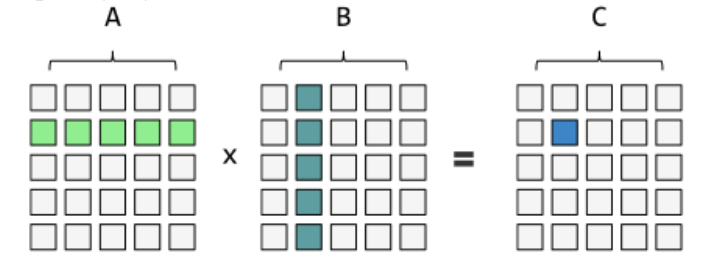
\includegraphics[scale=0.5]{./images/multiplicacion.png}
    \centering
    \caption{Multiplicación de matrices.}
    \label{fig:mult-matrices}
\end{figure}

La elección de este código es debida a que un gran porcentaje del código del problema de multiplicación de matrices por bloques es paralelizable (quitando la inicialización y liberación de memoria). El código se puede hacer escalar de forma sencilla, ya que podría llegar fácilmente a días de ejecución en la versión secuencial, dependiendo del tamaño de las matrices. Además, la multiplicación de matrices es un subproblema muy utilizado hoy en día en muchísimos otros problemas de mayor complejidad. Esto nos permite ver que este estudio tiene un gran sentido y podría tener un gran impacto sobre otros problemas.



\subsection{Análisis de Código Paralelizable}

Una vez que se tiene la versión secuencial, el primer código paralelo que se realizó fue el de OpenMP. Como hemos estudiado en la asignatura de Metodología de la Programación Paralela impartida por la Universidad de Murcia, antes de comenzar a realizar programación paralela hay que realizar un estudio sobre qué partes del código pueden ser paralelizables, y dentro de estas, cuáles merecen la pena, pues si dentro de una zona paralelizable hay una carga de trabajo muy pequeña, la sobrecarga que hay al dividir el trabajo en los hilos puede ser mayor que el paralelismo que se consigue, por lo que no merecería la pena.

En este estudio vemos qué partes del código se pueden paralelizar. Una vez revisado y estudiado el código  encontramos dos zonas en las que podemos implementar la paralización, la primera es un bucle dentro de la función {\it multPorBloques} donde se realiza la multiplicación de estos bloques (submatrices) como mencionamos. Como dijimos esta rutina {\it MMB} se eligió por el tema de la caché y, por tanto, el tamaño de los bloques dependerá del tamaño de esta. Tal como se verá con detalle en el Apartado~\ref{section:cache}, los mejores resultados se dan con bloques de tamaño 8$\times$8 y 16$\times$16, siendo el caso más grande una multiplicación de matrices de tamaño 16$\times$16. Esto nos daba un resultado que aunque mejoraba un poco los tiempos de ejecución, no era lo que buscábamos, pues en cada inicio de multiplicación habría que hacer un reparto del trabajo, siendo este reparto explícito en memoria distribuida o implícito en memoria compartida.

La otra zona que se observó que era paralelizable y que se puede ver en el  Algoritmo~\ref{alg:mult-matrices}, es un bucle de varias iteraciones en el que se termina llamando a la función de multiplicación por bloques mencionada anteriormente. De esta forma, el reparto de trabajo entre los distintos hilos o procesadores solo se realizará una vez durante toda la ejecución del programa. Además, engloba de forma completa la rutina {\it MMB}, consiguiendo de esta forma un paralelismo eficiente y una reducción del tiempo bastante considerable.

Teniendo ahora el código de la versión secuencial y la zona paralelizable de este en la que obtenemos buenos resultados, procedemos a implementarlos y ver qué opciones hemos tenido para la paralelización de este, tanto en paso de mensajes como en memoria compartida.

\subsection{Memoria Compartida}
\subsubsection{Programación mediante memoria compartida}
El primer método de programación paralela que vamos a ver consiste en que un procesador puede tener varios hilos ({\it threads}) que trabajan sobre la misma región de memoria, pudiendo leer y escribir sobre una zona de memoria compartida al mismo tiempo. Por ello, estos hilos son dependientes entre sí, aunque no necesitan programación especial para la coordinación, se deben comunicar a la hora de actualizar (escribir) las zonas de memoria compartida.


\begin{figure}[htbp]
    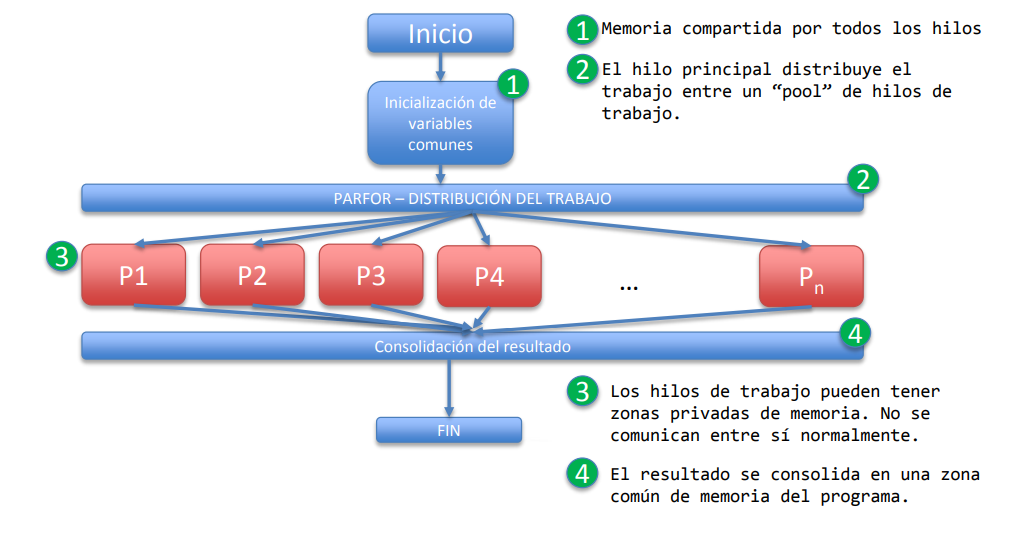
\includegraphics[scale=0.65]{./images/2.1.arte-omp.PNG}
    \centering
    \caption{Explicación gráfica de memoria compartida~\cite{icmat}.}
    \label{fig:arte-omp}
\end{figure}

Como podemos ver en la Figura~\ref{fig:arte-omp}, en primer lugar se inicializan en la memoria compartida del computador los datos que compartirán los distintos hilos. Durante su ejecución, a menos que se indique explícitamente, no se requerirá ninguna programación especial para la coordinación entre ellos, pero deben hacerlo en caso de que escriban en la misma zona  de memoria (variable compartida). Esto se debe a que si dos hilos realizan a la vez una escritura en la misma variable puede haber inconsistencias en los datos y, por tanto, puede incurrir en errores. Por ello, se suele intentar evitar el conflicto entre los hilos creando sus propias variables privadas, de forma que estos escriben sus resultados en sus propias variables durante la ejecución, y al final deben coordinarse para escribir el resultado final en las variables que se encuentran en memoria compartida.


Esta forma de programación, por lo tanto, saca mucho rendimiento cuando los hilos no entran en conflictos entre ellos a la hora de leer y escribir en la memoria compartida durante la ejecución del código paralelo. Si hay conflicto, los hilos se tendrán que sincronizar (bloquear) entre ellos, y formarán un cuello de botella siendo difícil cumplir lo que se busca con esta implementación, y es que el coste de sincronización de datos entre procesos más el coste de generación de procesos, sea menor al beneficio obtenido mediante el paralelismo.


\subsubsection{Implementación de la versión Paralela en Memoria Compartida} \label{section:imp-memCom}

La primera implementación de código paralelo la hemos realizado usando memoria compartida. Para comenzar, hemos trabajado con OpenMP con el cual ya habíamos trabajado en la asignatura de la universidad, con el objetivo de que el primer contacto nos fuera más sencillo. Una vez visto en el apartado anterior la zona de código donde podemos aplicar paralelización, el siguiente paso es ver qué forma es la más correcta dentro de las que estas librerías nos permiten para nuestro código.

En esta primera implementación hemos probado dos directivas diferentes que nos da como herramientas la librería de OpenMP. La primera sería mediante la utilización de tareas, es decir, habría un hilo principal creado con la directiva {\it single} que iría generando tareas en cada iteración del doble bucle {\it for} (recorrido de filas y columnas de submatrices de las matrices principales). Cada tarea se iría asignando a un hilo mediante la directiva {\it task}, siendo el trabajo de cada tarea la ejecución de varias multiplicaciones por bloque de submatrices que diese como resultado un solo bloque de submatriz resultante. Esto sería la secuencia que hemos visto en la Figura~\ref{fig:mult-matrices}. Esta implementación se puede visualizar en el Algoritmo~\ref{alg:single-task}, el cual es similar al Algoritmo~\ref{alg:mult-matrices} pero con la implementación explicada anteriormente.

\begin{algorithm} [htbp]
	\caption{Implementación paralela con OpenMP y las directivas {\it single-task}}
    \hspace*{\algorithmicindent} \textbf{Input} matA, matB, tamMat, tamSubMat\\
    \hspace*{\algorithmicindent} \textbf{Output} matC
	\begin{algorithmic}[1]
	    \State $numSubMatFilas \leftarrow tamMat/tamSubMat$
		\State $numSubMatCols \leftarrow tamMat/tamSubMat$
		\State \#pragma omp parallel
		\State \{
		\State \#pragma omp single
        \State \{
		\For {i = 0 to numSubMatFilas}
		\For {j = 0 to numSubMatCols}
	        \State \#pragma omp task 
            \State \{
			\For {k = 0 to numSubMatCols}
				\State $nSubMatA \leftarrow (i * numSubMatCols) + k$ 
				\State $nSubMatB \leftarrow  (k * numSubMatCols) + j$
				\State $nSubMatC \leftarrow  (i * numSubMatCols) + j$
				
				\State multPorBloques(matA, nSubMatA, matB, nSubMatB, matC, nSubMatC, tamMat, tamSubMat)
            \EndFor
	        \State \}
        \EndFor
		\EndFor
		\State \}
		\State \}
	\end{algorithmic}
	\label{alg:single-task}
\end{algorithm}

La segunda forma seria, al principio del doble bucle {\it for} (que se puede ver en el pseudocódigo del Algoritmo~\ref{alg:mult-matrices}), utilizar la directiva {\it parallel for} junto a {\it collapse}. De esta forma la primera directiva lo que nos permite es en un bucle {\it for} dividir las iteraciones, es decir, si tenemos 80 iteraciones y 8 hilos, cada hilo realiza 80/8~=~10 iteraciones, y junto a {\it collapse}, que lo que hace es si hay dos o más bucles {\it for} consecutivos, podemos definirlos como si hubiera uno solo, de forma que si tenemos dos bucles de 80 iteraciones cada uno, en total serian 6400 iteraciones. Siguiendo con el ejemplo anterior, si tenemos 8 hilos, cada hilo realizaría 6400/8~=~800 iteraciones. Esto hace que solo haya que realizar una vez (y no tantas como bucles haya) la división del trabajo para cada hilo. Esta implementación se puede visualizar en el  Algoritmo~\ref{alg:for-collapse}. Debido a esto último, este método es mejor que el anterior, pues es mejor repartir el trabajo una sola vez entre los hilos que estar generando tareas y hilos una y otra vez en cada iteración, dando lugar a que en cada iteración de los bucles haya una sobrecarga innecesaria en tiempo de ejecución.

\begin{algorithm}[htbp]
	\caption{Implementación paralela con OpenMP y las directivas {\it parallel for-collapse}}
    \hspace*{\algorithmicindent} \textbf{Input} matA, matB, tamMat, tamSubMat\\
    \hspace*{\algorithmicindent} \textbf{Output} matC
	\begin{algorithmic}[1]
	    \State $numSubMatFilas \leftarrow tamMat/tamSubMat$
		\State $numSubMatCols \leftarrow tamMat/tamSubMat$
		\State \#pragma omp parallel for collapse(2)
		\State \{
		\For {i = 0 to numSubMatFilas}
		\For {j = 0 to numSubMatCols}
			\For {k = 0 to numSubMatCols}
				\State $nSubMatA \leftarrow (i * numSubMatCols) + k$ 
				\State $nSubMatB \leftarrow  (k * numSubMatCols) + j$
				\State $nSubMatC \leftarrow  (i * numSubMatCols) + j$
				
				\State multPorBloques(matA, nSubMatA, matB, nSubMatB, matC, nSubMatC, tamMat, tamSubMat)
            \EndFor
        \EndFor
		\EndFor

		\State \}
	\end{algorithmic}
	\label{alg:for-collapse}
\end{algorithm}

Lo que acabamos de ver lo podemos extrapolar a la paralelización del código con Intel TBB. Investigando qué herramientas tiene para poder realizar lo que hemos hecho con OpenMP, encontramos que Intel TBB también tiene una llamada a {\it parallel for}, en la que podemos encadenar cuantos bucles {\it for} queramos, unos dentro de otros, utilizando de nuevo la misma llamada (diferencia respecto a OpenMP). En nuestro caso solo necesitamos dos, pero investigando un poco más, se encuentra que esta librería tiene las funciones {\it blocked range2d} y {\it blocked range3d}. En este trabajo hemos utilizado solo la primera, ya que en nuestro código solo encadenamos 2 bucles {\it for} de forma paralela. Esta función sería un sinónimo del {\it collapse} (aunque más completo, pues en {\it collapse} tienen que estar los bucles seguidos) de OpenMP, permitiendo que la iteraciones que hay en dos bucles {\it for} correctamente definidos se puedan repartir en una sola vez como si solo hubiera un bucle y haciendo de esta forma que mejore el tiempo de ejecución. Esta implementación se puede ver en el pseudocódigo del Algoritmo~\ref{alg:tbb}.


\begin{algorithm}[htbp]
	\caption{Implementación paralela con Intel TBB y el método {\it blocked range2d}}
    \hspace*{\algorithmicindent} \textbf{Input} matA, matB, tamMat, tamSubMat\\
    \hspace*{\algorithmicindent} \textbf{Output} matC
	\begin{algorithmic}[1]
	    \State $numSubMatFilas \leftarrow tamMat/tamSubMat$
		\State $numSubMatCols \leftarrow tamMat/tamSubMat$
		\State parallel\_for(blocked\_range2d(0, numSubMatFilas, 0, numSubMatCols), [\&](const blocked\_range2d  r)
		\State \{
		\For {i = r.rows().begin() r.rows().end()}
		\For {j = r.cols().begin() to r.cols().end()}
			\For {k = 0 to numSubMatCols}
				\State $nSubMatA \leftarrow (i * numSubMatCols) + k$ 
				\State $nSubMatB \leftarrow  (k * numSubMatCols) + j$
				\State $nSubMatC \leftarrow  (i * numSubMatCols) + j$
				
				\State multPorBloques(matA, nSubMatA, matB, nSubMatB, matC, nSubMatC, tamMat, tamSubMat)
            \EndFor
        \EndFor
		\EndFor
        \State \}
	\end{algorithmic}
	\label{alg:tbb}
\end{algorithm}

Como hemos ido mencionando en este documento, en memoria compartida el reparto del trabajo será implícito, es decir, no decidimos nosotros cómo se hace el reparto del trabajo entre los hilos, simplemente sabes que tanto OpenMP como IntelTBB nos garantizan que internamente el trabajo se ha dividido de forma correcta y de la forma más igualada posible entre los hilos. La forma para comprobar que nuestra implementación ha sido correcta es coger el secuencial, ejecutarlo con las mismas matrices multiplicadoras, y comparar las dos matrices resultantes viendo si hay alguna diferencia.

El código de la implementación de Intel TBB se puede ver con más detalles y con una implementación cercana a C++ en el Apéndice~\ref{app:A}.

\subsection{Memoria distribuida (paso de mensajes)}
\subsubsection{Programación mediante memoria distribuida}

En la programación mediante paso de mensajes (sistemas con memoria distribuida), cada proceso tiene solo su propia región de memoria, por tanto, no habrá conflictos a la hora de escribir en memoria como en memoria compartida, pues un proceso no puede acceder a la memoria de los otros procesos, solo a la suya. Esta es una de las principales ventajas de la memoria distribuida, pues cada proceso obtiene independencia y libertad al acceder a su memoria sin obtener conflictos en los accesos pudiendo realizar su ejecución de forma consistente.

\begin{figure}[htbp]
    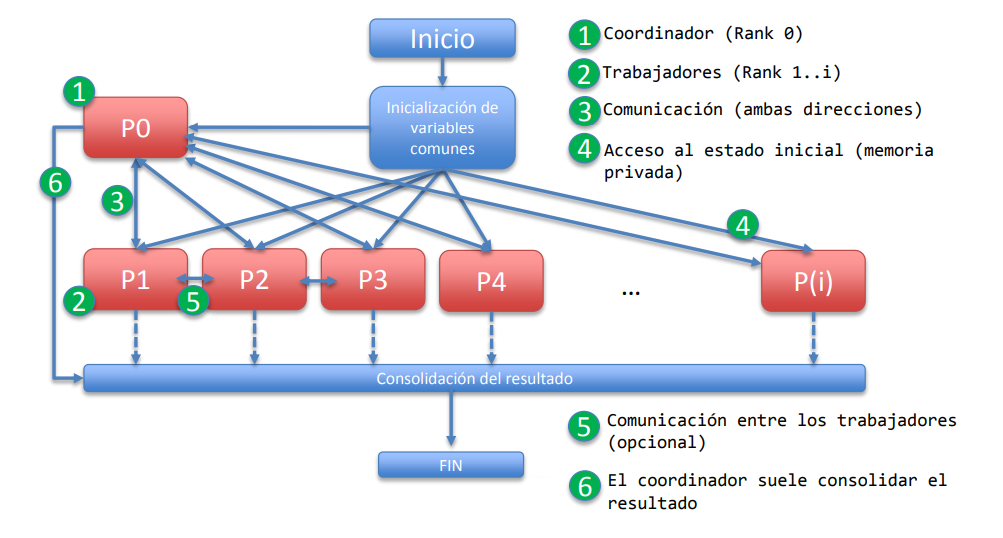
\includegraphics[scale=0.65]{./images/2.2.arte-mpi.PNG}
    \centering
    \caption{Explicación gráfica de paso de mensajes~\cite{icmat}.}
    \label{fig:arte-mpi}
\end{figure}



Como se puede observar en la  Figura ~\ref{fig:arte-mpi}, primero se inicializan las variables o datos comunes que tienen todos los procesos, pero a la vez independientes. Es decir, cada proceso tiene esas variables con los mismos datos pero en su propia región de memoria. Posteriormente, cada proceso puede modificar los valores de esas variables sin modificar el del resto de los procesos, pues cada variable está en una zona de memoria distinta, es decir, en memorias de distintos procesos.

Ahora viene la primera complicación, y es que, tiene que haber un proceso principal ({\it master}) que se encargue de repartir el trabajo con los demás. Este tiene que repartir el trabajo de forma manual, al contrario que en memoria compartida. Este proceso principal que suele ser el proceso 0 (en la imagen hace referencia a P0) debido a que siempre al menos estará un proceso activo y este tendrá el primer id asignable posible que es el número 0 (pues los procesos se asignan en orden desde 0 hasta num. procesos-1), así a falta de saber cuántos otros procesos tendrás, el proceso 0  siempre lo tendrás referenciado con un id que siempre existe, pudiendo repartir/recibir trabajo de una forma consistente con los otros procesos.

Ahora, el proceso 0 tiene además de las variables comunes (valores compartidos con los otros y no memoria), unas variables que él ha inicializado propiamente en su memoria para repartir, uno a uno o uno a muchos, a los demás procesos. De esta forma, el proceso 0 comunicará mediante mensajes esta información a los demás con la que les indicará el trabajo a realizar. Se hace de esta forma para que cada proceso tenga en su memoria su información individual y correspondiente sin tener que tener en su memoria información innecesaria, como por ejemplo, el trabajo de otro proceso. Esto es una ventaja como se puede ver, pues la ocupación de la memoria en cada proceso está optimizada, pero a la vez se necesita una coordinación entre los procesos para enviar y recibir los mensajes de forma correcta. Como inconveniente se tiene que el código se vuelve más complejo. 

Una vez que cada proceso ha finalizado su trabajo, este tiene que reunirse en el proceso 0. La forma será parecida a cuando se reparte, que es enviando mensajes uno a uno o todos a uno, siendo el receptor el proceso 0 y el emisor o emisores cualquiera de los otros procesos, o todos respectivamente (incluido el proceso 0 si son comunicaciones globales).

Estas comunicaciones no se tienen porque hacer solamente una vez durante la ejecución, es decir, puede haber varias comunicaciones entre los procesos y el proceso 0, ya sea para comunicarse con otros trabajos y resultados, o para abortar ejecuciones si por ejemplo el trabajo era una búsqueda recursiva que se ha dividido entre los distintos procesos y se ha encontrado el objetivo en uno, pues ya no se necesita continuar de la ejecución en los otros. Al final de este paso de mensajes, el proceso 0 será siempre (o como norma general) el que termine entregando el resultado que se ha obtenido como esfuerzo de todos los procesos.

La desventaja más grande, por ende, de esta metodología es que requiere una programación especial para la coordinación de mensajes que se envían durante la ejecución y, por ello, es necesario un conocimiento más amplio sobre este método para poder utilizarlo de forma correcta y eficaz. Por otro lado, su mayor ventaja es que si se consiguen comunicar bien los distintos procesos, resulta en que puedes tener 2 nodos (2 ordenadores) o más interconectados, de forma que cuando ejecutas un código paralelo entre estos se puede sacar la potencia de cómputo de todos los nodos que se tienen interconectados.

La eficiencia en este método está limitada a que los procesos puedan comunicarse de forma eficiente y al coste de los mensajes (cuanto más grande más tarda) enviados entre ellos. Por ello, se busca que el beneficio ganado por el paralelismo sea mayor que los dos inconvenientes mencionados anteriormente.

\subsubsection{Implementación en Memoria Distribuida}

Para la implementación en memoria distribuida hemos hecho igual que en el caso anterior, primero hemos trabajado y mirado en la versión de Open MPI, pues ya habíamos trabajado con ella en la asignatura. A diferencia de memoria compartida, en esta tenemos que dividir explícitamente la matriz A entre cada proceso para poder multiplicarla por la matriz B, y tener así como resultado la matriz resultante de la multiplicación. Por ello, el proceso principal (con id 0) se encarga de inicializar las dos matrices, tanto A como B. 

En una multiplicación de matrices, para sacar una fila de la matriz resultado, se multiplica una fila de A por todas las columnas de la matriz B. Igualmente ocurre en la multiplicación por bloques, para obtener una fila de submatrices de la matriz resultado, se multiplica una fila de submatrices de A, por todas las columnas de submatrices de B. Tal y como se explicó mediante la Figura~\ref{fig:mult-matrices} en el Apartado~\ref{seccion:secu}, vemos que la matriz B la tenemos que tener en todos los procesos, mientras que la matriz A, cada proceso solo tiene que tener las filas de las submatrices que le toca, no toda la matriz entera. Para hacer esto, haremos uso de la función {\it MPI\_BROADCAST}. Mediante esta función podemos propagar la matriz B desde el proceso 0 hasta el resto de los procesos. Luego se hará uso del método {\it MPI\_SCATTER} con el que se divide la matriz A, que tiene de momento solo el proceso 0 en porciones de filas, y se reparten entre todos los procesos (incluido el mismo) las filas de forma equitativa. Esta parte se puede ver en las líneas 1-16 del Algoritmo \ref{alg:mpi}.

\begin{algorithm}[htbp]
\caption{Implementación paralela mediante paso de mensajes con MPI}
\hspace*{\algorithmicindent} \textbf{Input} tamMat, tamSubMat, numProc\\
\hspace*{\algorithmicindent} \textbf{Output} matC
\begin{algorithmic}[1]


\State \textbf{MPI\_Init()}
\State $filasLocal \leftarrow tamMat/numProc$
\State $colsLocal \leftarrow tamMat$
\State $matALocal \leftarrow malloc(filasLocal$ $\times$ $colsLocal)$
\State $matCLocal \leftarrow malloc(filasLocal$ $\times$ $colsLocal)$
\State $matB \leftarrow malloc(tamMat$ $\times$ $tamMat)$

\If{$proc = 0$} 
    \State recibe o crea matA
    \State recibe o crea matB
    \State \textbf{MPI\_Bcast}(matB, tamMat$\times$tamMat, MPI\_INT, 0, MPI\_COMM\_WORLD)
    \State \textbf{MPI\_Scatter}(matA, filasLocal$\times$colsLocal, MPI\_INT, matALocal, filasLocal$\times$colsLocal, MPI\_INT, 0, MPI\_COMM\_WORLD)
\Else
    \State \textbf{MPI\_Bcast}(matB, tamMat$\times$tamMat, MPI\_INT, 0, MPI\_COMM\_WORLD)
    \State \textbf{MPI\_Scatter}(matA, filasLocal$\times$colsLocal, MPI\_INT, matALocal, filasLocal$\times$colsLocal, MPI\_INT, 0, MPI\_COMM\_WORLD)
\EndIf 

\State $numSubMatFilas \leftarrow filasLocal/tamSubMat$
\State $numSubMatCols \leftarrow colsLocal/tamSubMat$

\For {i = 0 to numSubMatFilas}
\For {j = 0 to numSubMatCols}
\For {k = 0 to numSubMatCols}
	\State $nSubMatA \leftarrow (i * numSubMatCols) + k$ 
	\State $nSubMatB \leftarrow  (k * numSubMatCols) + j$
	\State $nSubMatC \leftarrow  (i * numSubMatCols) + j$
	
	\State multPorBloques(matALocal, nSubMatA, matB, nSubMatB, matCLocal, nSubMatC, tamMat, tamSubMat)
\EndFor
\EndFor
\EndFor
\If{$proc = 0$} 
    \State \textbf{MPI\_Gather}(matCLocal, filasLocal$\times$colsLocal, MPI\_INT, matC, filasLocal$\times$colsLocal, MPI\_INT, 0, MPI\_COMM\_WORLD)
\Else
    \State \textbf{MPI\_Gather}(matCLocal, filasLocal$\times$colsLocal, MPI\_INT, null, filasLocal$\times$colsLocal, MPI\_INT, 0, MPI\_COMM\_WORLD)
\EndIf 
\State \textbf{MPI\_Finalize()}
\end{algorithmic}
\label{alg:mpi}
\end{algorithm}

Una vez hecha esta división, cada proceso realizará su trabajo como en el caso secuencial, hará la rutina {\it MMB} de la parte que le toca y obtendrá sus filas de submatrices de la matriz resultado. Después, le tocará de nuevo comunicarse con el proceso 0 para entregarle estas filas que ha calculado. Para ello, todos los procesos (incluido el proceso 0) llamarán a la función {\it MPI\_GATHER} con la que reunirán el trabajo realizado en el proceso 0 dando lugar a la matriz resultado completa y terminando así la ejecución del programa. El pseudocódigo de esta última parte se encuentra en las líneas 17-33 del Algoritmo~\ref{alg:mpi} que hemos mencionado anteriormente.

Si comparamos el conjunto de funciones que ofrecen las librerías Open MPI e Intel MPI, podemos observar que las llamadas a las funciones que contienen tienen los mismos nombres, aunque luego internamente trabajan de forma distinta. Debido a ese motivo, la implementación ha sido la misma en Open MPI y en Intel MPI. La única diferencia, a primera vista, es en la compilación como ya veremos, además de las librerías como hemos mencionado. Estas diferencias se podrán visualizar en los tiempos de ejecución que más adelante se verán en la comparación entre las dos. Por tanto, el pseudocódigo mostrado en el Algoritmo~\ref{alg:mpi} sirve tanto para Open MPI como para Intel MPI.

Una implementación más detallada cercana al lenguaje C++ se puede encontrar en el Apéndice~\ref{app:B}, siendo la implementación de Intel MPI pero que también nos sirve para Open MPI pues es la misma implementación como hemos dicho.

\subsection{Modelo híbrido de la programación paralela}
\subsubsection{Introducción a la programación híbrida}
Este método de programación paralela que vamos a ver y estudiar es, en resumen, una mezcla de los dos métodos anteriores. Trata de obtener los puntos fuertes de cada método de forma que te permite optimizar un poco más la ejecución de un programa.


Este paradigma se centra en aplicar dos niveles de programación. La primera capa alta consistiría en aplicar la memoria distribuidas, en la que habríamos repartido el trabajo a realizar a cada proceso en su memoria. Tras ello, aplicaríamos por debajo el segundo nivel de paralelismo que consistiría en utilizar el paradigma de memoria compartida, en la que, dentro de cada proceso, podremos generar hilos, de forma que la ejecución que antes era secuencial dentro de cada proceso ahora se haga de forma paralela al aplicarle este segundo nivel de programación.

Aunque esta forma en principio puede parecer muy eficiente, la verdad es que puede tener un sobrecoste a la hora de tener que crear los distintos procesos, tanto de memoria compartida como en el caso de paso de mensajes. Además, sigue teniendo los mismos inconvenientes de los dos métodos anteriores. En el paso de mensajes seguirá teniendo la complicación y coste adicional de los mensajes entre los distintos procesos, y en el caso de memoria compartida, la sincronización entre los hilos dentro de cada proceso.

Por estos motivos, a veces no es el método más eficaz entre los aquí estudiados, y en vez de mejorar el rendimiento lo que hace es empeorarlo. Además, supone una complicación más a la hora de programar paralelamente.

Por todo lo anterior, lo que se intenta cumplir en este paradigma es una combinación de las dos ideas anteriores. Es decir, que el coste de la sincronización entre los hilos de la memoria compartida, más el coste de la transmisión de los mensajes en memoria distribuida, más el coste de generación de procesos, sea menor que el beneficio ganado con el paralelismo.

\subsubsection{Implementación de la versión híbrida}

La implementación de la versión híbrida, en este caso, es una mezcla de las dos versiones anteriores, tanto la de Open como la de Intel. Tal y como se explica en la introducción,  primero aplicamos un primer nivel de programación paralelo mediante pasos de mensajes en el que utilizamos Open MPI o Intel MPI dependiendo si estamos usando las librerías de Open o Intel para repartirnos las filas de la matriz A que multiplicará cada proceso. Luego en la parte en la que se ejecutaba secuencialmente la rutina {\it MMB} aplicamos un segundo nivel de programación paralela con memoria compartida mejorando el rendimiento en esta parte. Usamos las directivas de OpenMP ({\it parallel for} junto a {\it collapse}) para el híbrido de Open o las funciones de Intel TTB ({\it blocked range2d}) para el híbrido de Intel. Estas directivas y funciones han sido también las que se han mencionado en la implementación de la memoria compartida en el Apartado~\ref{section:imp-memCom}. Resultando en que el código del híbrido de Open sea una mezcla entre los pseudocódigos que hemos ya hemos visto que son el Algoritmo~\ref{alg:mpi} en un primer nivel y el Algoritmo ~\ref{alg:for-collapse} en el segundo nivel. De la misma forma, el híbrido de Intel sería una mezcla entre el Algoritmo~\ref{alg:mpi} y el Algoritmo ~\ref{alg:tbb} del primer y segundo nivel de la implementación híbrida respectivamente.

\subsection{Selección del Tamaño de Bloque}
\label{section:cache}

Cuando un dato es copiado desde la memoria RAM hacia la memoria caché, también se copian los datos contiguos en memoria (mismo bloque de caché). Esto es relevante porque en nuestro código cuando traemos un número de una matriz, también traemos los datos contiguos aprovechando la localidad espacial, es decir, treaemos la fila (entera o parcial) donde está ese dato. En el caso de la matriz A no hay problema porque el recorrido se hace por filas, pero en el caso de la matriz B, el recorrido se hace por columnas y, por ello, se produce un fallo de caché en cada iteración de la multiplicación (considerando matrices de dimensiones grandes). Por este motivo, la multiplicación por bloques reduce el tiempo de ejecución, debido a que si se pueden mantener dos submatrices en caché, sin que ninguna fila tenga que salir de esta, los fallos se reducirán o prácticamente serán nulos una vez las matrices estén en ella, reduciendo de esta forma los accesos a memoria principal y, por ello, el tiempo de ejecución del programa.

Para conseguir el objetivo de que las dos submatrices quepan en la caché se tiene que elegir correctamente el tamaño de estas submatrices, que también dependerán de lo que pueda albergar la caché de cada CPU o nodo. Además, antes de ir a disco comprueba si el dato está en memoria RAM, por lo cual, también tiene importancia su tamaño. Los tiempos de ejecución que vamos a mostrar en este estudio se han realizado en el nodo Venus del clúster que nos proporciona la universidad. Este nodo posee 64 GB de memoria RAM, y caches L1 y L2 privadas por core de 32 KB y 256 KB respectivamente. Para nuestro cálculo estos datos son los más importantes y, en especial, el tamaño de la caché L1, aunque en un análisis más avanzado también se podrían necesitar los otros elementos del clúster. La fórmula para saber entonces el tamaño de bloque adecuado sería:

%El aviso es debido a la ñ de las palabras
\begin{equation} \label{equ:cache}
 3 \times (tamañoDeBloque) ^ 2 \times tamañoElemento = tamañoCache
\end{equation}

En nuestro caso, {\it tamañoElemento} es 4 bytes debido a que las matrices son de tipo entero ({\it int}). Nótese que se multiplica por 3 debido a que es necesario que quepan 3 submatrices (bloques), las dos matrices que multiplican y la matriz donde se escribe el resultado. Despejando los valores quedaría en que:


\[tamañoBloque = \sqrt{32KB/(4B \times 3)}\]
\[tamañoBloque = 51,63\]

Poniéndolo en potencia de 2, el tamaño más próximo de submatrices que pudiera mantenerse en cache seria de 32$\times$32. Este seria el modelo teórico y ahora vamos a comprobar que bloque es el más correcto, primero en Venus con matrices de 2048$\times$2048, utilizando 4 hilos en memoria compartida, 4 procesos en memoria distribuida y 2 de cada en los  híbridos, estos tiempos se pueden ver en la siguiente tabla:


\begin{table}[htbp]
\begin{NiceTabular}{cccccccc}[hvlines]
\CodeBefore
   \columncolor[HTML]{FAEBD7}{1}
   \columncolor[HTML]{FBCEB1}{2}
   \columncolor[HTML]{FF9966}{3,4,5}
   \columncolor[HTML]{A2A2D0}{6,7,8}
\Body
\Block{2-1}{\textbf{Tam.} \\ \textbf{SubMat.}} & \Block{2-1}{\textbf{Secuencial}} & \Block{2-1}{\textbf{Open}  \\ \textbf{OMP}} & \Block{2-1}{\textbf{Open} \\ \textbf{MPI} } & \Block{2-1}{\textbf{Open} \\ \textbf{Hib.}}  & \Block{2-1}{\textbf{Intel} \\ \textbf{TBB}}& \Block{2-1}{\textbf{Intel} \\ \textbf{MPI}} & \Block{2-1}{\textbf{Intel} \\ \textbf{Hib.}} \\
 & & & & & & & \\    
4   & 226,18  & 77,61 & 50,89  & 61,07  & 70,03 & 60,42 & 57,36 \\ 
8   & 80,32   & 27,93 & 20,98  & 21,59  & 42,31 & 31,93 & 33,49  \\ 
16  & 76,68   & 26,58 & 19,72  & 21,21  & 28,1  & 24,55 & 24,67 \\ 
32  & 135,31  & 35,58 & 34,96  & 34,99  & 39,01 & 37,92 & 38,12 \\ 
64  & 132,43  & 33,78 & 33,95  & 34,27  & 34,83 & 34,98 & 34,96 \\ 
128 & 129,61  & 33,56 & 33,2   & 33,22  & 33,91 & 34,08 & 34,09 \\ 
256 & 128,56  & 32,91 & 32,87  & 32,96  & 33,61 & 33,7  & 33,54 \\ 
\end{NiceTabular}
\caption{\label{tab:cache}\centering Comparativa de tiempos de ejecución (seg) de la rutina {\it MMB} en el nodo Venus con matrices de 2048$\times$2048 para distintos tamaño de bloque entre las distintas implementaciones.}
\end{table}

Como se puede ver en la Tabla~\ref{tab:cache}, el tamaño de bloque que mejores resultados obtiene en el nodo Venus ha sido el de 16$\times$16 en todas las implementaciones utilizadas. Teóricamente debería de haber sido el de 32, pero este no es el correcto debido a que además de las matrices puede haber otros datos o subrutinas que hagan uso de la caché, haciendo que el bloque teórico calculado se quedara grande, y siendo en la practica el bloque de tamaño 16$\times$16 el más eficiente. No se entrará más a fondo en este estudio, aunque es interesante, pues puede influir de una forma importante en los tiempos de ejecución como se ha podido ver. La finalidad principal de este era elegir el tamaño de bloque más eficiente a utilizar para las ejecuciones en las comparaciones de los siguientes apartados.


\subsection{Análisis de Prestaciones}
En esta sección vamos a realizar la comparación entre las diferentes alternativas que hemos ido mencionando en el documento, para ver cuál es la que ofrece mejores resultados.


\subsubsection{Configuración}
Para las siguientes comparaciones hemos utilizado un nodo llamado Venus del clúster proporcionado por la Facultad de Informática de la Universidad de Murcia. Las características de este nodo que nos mencionan son las siguientes:

El nodo de cómputo Venus tiene 2 CPU's Intel Xeon E5-2620 (hexa-core) que funcionan a una frecuencia de 2.40 GHz y tienen una arquitectura x86-64. Dispone de una arquitectura de memoria tipo NUMA con 64 GB de memoria RAM, caches L1 y L2 privadas por core de 32 KB y 256 KB, respectivamente, y una caché L3 de 15 MB compartida por todos los cores de cada socket (NUMA-Node). Dispone de una GPU NVIDIA GeForce GT 640 (Kepler) con 1024 MB de Memoria Global y 384 CUDA cores (2 Streaming Multiprocessors y 192 Streaming Processors por SM), y dos coprocesadores Intel Xeon Phi3120A Knights Corner con 57 cores físicos (228 lógicos) a 1,10 GHz, 6 GB de memoria y caches L1 y L2 privadas por core de 32 KB y 28.50 MB, respectivamente.

Además, como se mostró en el Apartado \ref{section:cache},  el mejor tamaño de submatriz para este nodo es de 16$\times$16, este tamaño de bloque será el que se utilizará en las comparaciones de los siguientes apartados. Respecto a los tiempos de ejecución que se mostraran, los códigos se han ejecutado varias veces y se ha hecho una media de los tiempos quitando los valores atípicos para que estos sean lo más justos posibles.

\subsubsection{OpenMP vs. Intel TBB}
\label{section:ompvstbb}
La primera comparativa que vamos a ver va a ser la de OpenMP con Intel TBB, siendo éstas dos librerías que se usan para la programación paralela en memoria compartida. Como se puede observar en la Tabla~\ref{tab:eje_mem}, la comparación se ha hecho con distintos tamaños de problema, distintos números de hilos y tomando el tiempo de ejecución secuencial como referencia. También hay que añadir que la compilación de los programas hay sido mediante {\it g++} y con la opción de optimización {\it -03} que dispone el compilador, pudiendo visualizar a continuación la compilación completa que hemos utilizado para los dos códigos:

- OpenMP: \texttt{g++ -O3 -std=c++1 omp.cpp 1 -o omp -fopenmp}

- Intel TBB: \texttt{g++ -O3 -std=c++11 tbb.cpp  -o tbb -ltbb}

Y la ejecución siendo: 

- OpenMP: \texttt{./omp .. Parámetros de entrada}

- Intel TBB: \texttt{./tbb .. Parámetros de entrada}

Siendo los parámetros de entrada el número de hilos, el tamaño del problema (matrices) y el tamaño de bloque (submatrices).
\begin{table}[htbp]
\begin{NiceTabular}{cccccccc}[hvlines]
\CodeBefore
   \columncolor[HTML]{FAEBD7}{1}
   \columncolor[HTML]{FBCEB1}{2}
   \columncolor[HTML]{FF9966}{3,4,5}
   \columncolor[HTML]{A2A2D0}{6,7,8}
\Body
\Block{2-1}{\textbf{Tam.} \\ \textbf{Mat.}}&\Block{2-1}{\textbf{Secuencial}} & \Block{1-3}{\textbf{OpenMP (hilos)}} &&& \Block{1-3}{\textbf{Intel TBB (hilos)}}  \\
&& \textbf{2hilos} & \textbf{4hilos} & \textbf{8hilos} & \textbf{2hilos} & \textbf{4hilos} & \textbf{8hilos} \\
512  & 0,117 & 0,074 & 0,038 & 0,025 & 0,074 & 0,041 & 0,025 \\
1024 & 1,057 & 0,548 & 0,296 & 0,175 & 0,536 & 0,291 & 0,163 \\ \hline
2048 & 8,794 & 4,599 & 2,511 & 1,439 & 4,493 & 2,371 & 1,394 \\ \hline
4096 & 77,62 & 45,48 & 26,95 & 18,39 & 41,64 & 24,37 & 15,18 \\ \hline
8192 & 807,1 & 442,4 & 250,4 & 178,3 & 433,1 & 235,8 & 155,7 \\ \hline
\end{NiceTabular}
\caption{\label{tab:eje_mem}\centering Comparativa de tiempos de ejecución (seg) de la rutina {\it MMB} en el nodo Venus con submatrices de 16$\times$16 y distintos num. de hilos entre OpenMP e Intel TBB.}
\end{table}

En la Tabla~\ref{tab:eje_mem} se puede observar que el tiempo de ejecución del programa que usa la librería OpenMP es mayor al que usa la librería Intel TBB. Esto se ve de forma más clara conforme se aumenta el tamaño del problema (tamaño de las matrices) en la rutina {\it MMB}. Esto se debe a que, además de que cuanto más grande es un problema (por lo general), mejor se visualizan las diferencias, a que también al ser más grande hay mayor carga en los hilos, y aquí es donde tiene que destacar cada librería, desde la creación de los hilos y su asignación del trabajo, hasta en la ejecución de este y la terminación del hilo.

\begin{table}[htbp]
\centering
\begin{NiceTabular}{ccccccc}[hvlines]
\CodeBefore
\rectanglecolor[gray]{0.8}{1-2}{1-7}
\rectanglecolor[gray]{0.8}{1-1}{3-1}
\rectanglecolor[HTML]{FF9966}{4-1}{8-1}
\rectanglecolor[HTML]{FAEBD7}{2-2}{8-4}
\rectanglecolor[HTML]{FBCEB1}{2-5}{8-7}
\Body
\Block{3-1}{\textbf{Tam.} \\ \textbf{Mat.}} & \Block{1-6}{\textbf{Speed-up obtenido en mem. compartida}}   \\
 &\Block{1-3}{\textbf{OpenMP}} &&& \Block{1-3}{\textbf{Intel TBB}}\\
& \textbf{2 hilos} & \textbf{4 hilos} & \textbf{8 hilos} & \textbf{2 hilos} & \textbf{4 hilos} & \textbf{8 hilos}\\
512  & 1,581 & 3,079 & 4,680 & 1,581 & 3     & 4,680  \\
1024 & 1,929 & 3,512 & 6,254 & 1,972 & 3,632 & 6,525  \\ 
2048 & 1,912 & 3,502 & 6,277 & 1,957 & 3,709 & 6,363  \\ 
4096 & 1,707 & 2,983 & 4,425 & 1,835 & 3,185 & 5,113  \\ 
8192 & 1,826 & 3,208 & 4,527 & 1,869 & 3,437 & 5,184  \\ 
\end{NiceTabular}
\caption{\label{tab:speed_mem}\centering {\it Speed-up} que se consigue con OpenMP e Intel TBB con las diferentes configuraciones respecto al tiempo de ejecución obtenido en el secuencial en la rutina {\it MMB} ejecutada en el nodo Venus.}
\end{table}


Esta mejora en los tiempos de ejecución de la librería Intel TBB respecto a OpenMP, que se puede observar en la Tabla~\ref{tab:eje_mem}, se puede visualizar también en la Tabla~\ref{tab:speed_mem}, donde se ven los {\it speed-up} obtenidos de ambos respecto al secuencial. En ella se puede ver que, efectivamente, cuanto mayor es el tamaño de problema y más hilos se utilizan, Intel TBB funciona mejor que OpenMP, aumentando también en los dos casos el {\it speed-up} conforme aumenta el número de hilos.


\subsubsection{Open MPI vs Intel MPI}
\label{section:mpivsimpi}
Open MPI e Intel MPI son dos librerías que se usan en la programación paralela mediante paso de mensajes (memoria distribuida). Para esta comparativa, también se han utilizado distintos tamaños de matrices y, en este caso, distinto número de procesos, con el tamaño de submatriz de 16$\times$16 que vimos y con el tiempo de referencia del secuencial como se puede ver en la Tabla~\ref{tab:eje_mpi}. En este caso, se utilizan distintos comandos de compilación, aunque por debajo acaba siendo el mismo compilador, que es {\it g++}. Los comandos utilizados para compilar ambos códigos se pueden ver a continuación:

- Open MPI:\texttt{mpic++ -O3 -std=c++1 mpi.cpp 1 -o mpi -fopenmp}

- Intel MPI: \texttt{mpicxx -O3 -std=c++11 impi.cpp  -o impi -ltbb}

Y la ejecución siendo: 

- Open MPI: \texttt{mpirun -n (Num.Proc.) ./mpi .. Parámetros de entrada}

- Intel MPI: \texttt{mpirun -n (Num.Proc.) ./impi .. Parámetros de entrada}

Los parámetros de entrada serían en este caso el tamaño del problema (matrices) y el tamaño del bloque (submatrices), pues no hay hilos y el número de procesos se tiene que poner antes junto a la opción {\it -n} de {\it mpirun}.
\begin{table}[htbp]
\begin{NiceTabular}{cccccccc}[hvlines]
\CodeBefore
   \columncolor[HTML]{FAEBD7}{1}
   \columncolor[HTML]{FBCEB1}{2}
   \columncolor[HTML]{FF9966}{3,4,5}
   \columncolor[HTML]{A2A2D0}{6,7,8}
\Body
\Block{2-1}{\textbf{Tam.} \\ \textbf{Mat.}}&\Block{2-1}{\textbf{Secuencial}} & \Block{1-3}{\textbf{Open MPI (procesos)}} &&& \Block{1-3}{\textbf{Intel MPI (procesos)}}  \\
&& \textbf{2proc.} & \textbf{4proc.} & \textbf{8proc.} & \textbf{2proc.} & \textbf{4proc.} & \textbf{8proc.} \\
512  & 0,117 & 0,071 & 0,038 & 0,022 & 0,072 & 0,038 & 0,021 \\ \hline
1024 & 1,057 & 0,562 & 0,298 & 0,185 & 0,575 & 0,322 & 0,182 \\ \hline
2048 & 8,794 & 4,618 & 2,334 & 1,366 & 4,407 & 2,344 & 1,352 \\ \hline
4096 & 77,62 & 38,65 & 19,58 & 11,13 & 38,06 & 19,48 & 11,11 \\ \hline
8192 & 807,1 & 402,5 & 203,9 & 114,7 & 400,4 & 203,6 & 114,5 \\ \hline
\end{NiceTabular}
\caption{\label{tab:eje_mpi}\centering Comparativa de tiempos de ejecución (seg) de la rutina {\it MMB} en el nodo Venus con submatrices de 16$\times$16 y distintos num. de procesos entre Open MPI e Intel MPI.}
\end{table}

En esta comparativa, los tiempos de ejecución que se consiguen con las dos implementaciones son muy parecidos tal y como se puede ver en la Tabla~\ref{tab:eje_mpi}. Aunque hay una pequeña tendencia conforme aumenta el tamaño del problema y procesos de Open MPI hacia Intel MPI, de forma que con tamaños pequeños funciona mejor Open MPI y conforme las comunicaciones entre los procesos empiezan a ser más costosas, debido a que las matrices que se envían son de mayor tamaño, Intel MPI recupera el terreno que le sacaba Open MPI, e incluso parece que lo mejora un poco, quedando finalmente de forma muy pareja. Aún así, la ganancia respecto a Open MPI es prácticamente inexistente. Todo lo mencionado anteriormente se puede ver de otra forma en la Tabla~\ref{tab:speed_dis}. Donde se ve que los {\it speed-up} de las dos implementaciones respecto a la versión secuencial son básicamente idénticos.

\begin{table}[htbp]
\centering
\begin{NiceTabular}{ccccccc}[hvlines]
\CodeBefore
\rectanglecolor[gray]{0.8}{1-2}{1-7}
\rectanglecolor[gray]{0.8}{1-1}{3-1}
\rectanglecolor[HTML]{FF9966}{4-1}{8-1}
\rectanglecolor[HTML]{FAEBD7}{2-2}{8-4}
\rectanglecolor[HTML]{FBCEB1}{2-5}{8-7}
\Body
\Block{3-1}{\textbf{Tam.} \\ \textbf{Mat.}} & \Block{1-6}{\textbf{ Speed-up obtenido en mem. distribuida}}   \\
 &\Block{1-3}{\textbf{Open MPI}} &&& \Block{1-3}{\textbf{Intel MPI}}\\
& \textbf{2 proc.} & \textbf{4 proc.} & \textbf{8 proc.} & \textbf{2 proc.} & \textbf{4 proc.} & \textbf{8 proc.}\\
512  & 1,671 & 3,079 & 5,318 & 1,625 & 3,079 & 5,571  \\
1024 & 1,922 & 3,547 & 5,714 & 1,838 & 3,283 & 5,808  \\ 
2048 & 1,904 & 3,768 & 6,438 & 1,995 & 3,752 & 6,504  \\ 
4096 & 2,008 & 3,964 & 6,974 & 2,039 & 3,985 & 6,986  \\ 
8192 & 2,005 & 3,958 & 7,037 & 2,016 & 3,964 & 7,049  \\ 
\end{NiceTabular}
\caption{\label{tab:speed_dis}\centering {\it Speed-up} que se consigue con Open MPI e Intel MPI con las diferentes configuraciones respecto al tiempo de ejecución obtenido en el secuencial en la rutina {\it MMB} ejecutada en el nodo Venus.}
\end{table}

\subsubsection{Versión híbrida de Open vs híbrido de Intel}
Esta última comparativa debería ser teóricamente una mezcla de los resultados de los apartados anteriores, ya que estas versiones híbridas son la mezcla de implementar memoria distribuida mediante Open MPI o Intel MPI junto a memoria compartida mediante OpenMP o Intel TBB. Como en las secciones anteriores, se utiliza una comparación usando submatrices de 16$\times$16, diferentes tamaños de problema y tomando el tiempo de la versión secuencial como referencia, todo ello se puede ver en la Tabla~\ref{tab:eje_hib}. Para la consecución de esos tiempos se ha compilado el código de los programas de la siguiente forma:

- Open híbrido: \texttt{mpic++ -O3 -std=c++1 hib.cpp 1 -o hib -fopenmp}

- Intel híbrido: \texttt{mpicxx -O3 -std=c++11 ihib.cpp  -o ihib -ltbb}

Y la ejecución siendo: 

- Open híbrido: \texttt{mpirun --bind-to none -n (Num.Proc.) ./hib .. Parámetros de entrada}

- Intel híbrido: \texttt{mpirun -n (Num.Proc.) ./ihib .. Parámetros de entrada} 

En este caso, en los parámetros va el numero de hilos que se ejecutan dentro de cada proceso (su cantidad se indican en la opcion {\it -n} de {\it mpirun}), el tamaño de problema (matrices) y el tamaños de bloque (submatrices).

\begin{table}[htbp]
\begin{NiceTabular}{cccccccc}[hvlines]
\CodeBefore
   \columncolor[HTML]{FAEBD7}{1}
   \columncolor[HTML]{FBCEB1}{2}
   \columncolor[HTML]{FF9966}{3,4,5}
   \columncolor[HTML]{A2A2D0}{6,7,8}
\Body
\Block{2-1}{\textbf{Tam.} \\ \textbf{Mat.}}&\Block{2-1}{\textbf{Secuencial}} & \Block{1-3}{\textbf{Open Hib. (proc-hilos)}} &&& \Block{1-3}{\textbf{Intel Hib. (proc-hilos)}}  \\
&& \textbf{2p, 2h} & \textbf{2p, 4h} & \textbf{4p, 2h} & \textbf{2p, 2h} & \textbf{2p, 4h} & \textbf{4p, 2h} \\
512  & 0,117 & 0,051 & 0,034 & 0,032 & 0,041 & 0,027 & 0,027 \\ \hline
1024 & 1,057 & 0,335 & 0,179 & 0,186 & 0,315 & 0,173 & 0,175 \\ \hline
2048 & 8,794 & 2,704 & 1,742 & 1,629 & 2,312 & 1,308 & 1,394 \\ \hline
4096 & 77,62 & 22,19 & 13,33 & 12,46 & 19,79 & 11,03 & 11,18 \\ \hline
8192 & 807,1 & 212,1 & 119,3 & 117,7 & 205,2 & 115,2 & 115,3 \\ \hline
\end{NiceTabular}
\caption{\label{tab:eje_hib}\centering Comparativa de tiempos de ejecución (seg) de la rutina {\it MMB} en el nodo Venus con submatrices de 16$\times$16 y distintas configuraciones de número de procesos y de hilos entre los híbridos de Open e Intel.}
\end{table}

Teóricamente, en este caso, tendríamos que haber obtenido una mezcla entre los tiempos de las dos anteriores comparativas. En el caso en el que Open iba mejor o igual que Intel con los tamaños de problema más pequeños. 

La Tabla~\ref{tab:eje_hib} nos muestra que el híbrido de Intel funciona bastante mejor al principio, haciendo una diferencia con las comparaciones anteriores. Esto no se debe a que el híbrido de Intel mejore con respecto a sus implementaciones individuales, sino a que el híbrido de Open, cuando mezclas OpenMP junto a Open MPI empeora, o por lo menos cuando no es un tamaño de problema grande, ya que cuando el problema de tamaño es el más grande sí que tiene un tiempo de ejecución más parecido al de Intel. Todo ello se puede deber a que el coste en la comunicación y la generación de hilos, en Open es más caro que en Intel y, cuando el tamaño del problema es pequeño, este es igual a que cuando es más grande, por lo que cuanto más grande es el problema, este sobrecoste en el tiempo se diluye de forma que se acerca al tiempo de Intel. Esto se puede ver de otra forma en la Tabla~\ref{tab:speed_hib}, donde vemos que el híbrido de Intel obtiene un speed-up mayor que el híbrido de Open en todas las comparaciones.

\begin{table}[htbp]
\centering
\begin{NiceTabular}{ccccccc}[hvlines]
\CodeBefore
\rectanglecolor[gray]{0.8}{1-2}{1-7}
\rectanglecolor[gray]{0.8}{1-1}{3-1}
\rectanglecolor[HTML]{FF9966}{4-1}{8-1}
\rectanglecolor[HTML]{FAEBD7}{2-2}{8-4}
\rectanglecolor[HTML]{FBCEB1}{2-5}{8-7}
\Body
\Block{3-1}{\textbf{Tam.} \\ \textbf{Mat.}} & \Block{1-6}{\textbf{Speed-up obtenido en las versiones híbridas}}   \\
 &\Block{1-3}{\textbf{Open Hib. (proc-hilos)}} &&& \Block{1-3}{\textbf{Intel Hib. (proc-hilos)}}\\
& \textbf{2p, 2h} & \textbf{2p, 4h} & \textbf{4p, 2h} & \textbf{2p, 2h} & \textbf{2p, 4h} & \textbf{4p, 2h} \\
512  & 2,340 & 3,441 & 3,656 & 2,854 & 4,333 & 4,333 \\
1024 & 3,155 & 5,905 & 5,683 & 3,356 & 6,110 & 6,040 \\ 
2048 & 3,252 & 5,326 & 5,398 & 3,804 & 6,723 & 6,308 \\ 
4096 & 3,498 & 5,823 & 6,230 & 3,920 & 7,037 & 6,943 \\ 
8192 & 3,807 & 6,765 & 6,857 & 3,933 & 7,006 & 7 \\ 
\end{NiceTabular}
\caption{\label{tab:speed_hib}\centering {\it Speed-up} que se consigue con el híbrido de Open y el híbrido de Intel con las diferentes configuraciones respecto al tiempo de ejecución obtenido en el secuencial en la rutina {\it MMB} ejecutada en el nodo Venus.}
\end{table}


\subsection{Uso de la herramienta de profiling Intel VTune}

Con el fin de esclarecer los resultados obtenidos en la comparativa de la sección anterior, entre las distintas librerías paralelas, se hace uso de la herramienta {\it profiling} Intel VTune~\cite{vtune}. En concreto, se ha usado su análisis llamado {\it threading}. Dicho análisis está hecho para analizar cómo se comportan programas paralelos como el nuestro. Con esto podemos obtener una segunda comparación que no se fije solo en el tiempo global de la ejecución, sino también en otros detalles que nos ofrece esta herramienta como son por ejemplo los tiempos de bloqueos entre los hilos o el tiempo que no se están usando todos los hilos o procesos. De esta forma, con las posibilidades que nos ofrece esta herramienta, podemos dar una mejor explicación a las diferencias de tiempos que hemos visto en el apartado anterior.

\subsubsection{Configuración}
Para esta comparación, se ha utilizado el ordenador del alumno debido a que esta herramienta no está instalada en el clúster y, además, la aplicación gráfica nos muestra un análisis más completo que con su uso en el terminal. Por ello, primero vamos a introducir las características del ordenador para saber con qué herramientas se está haciendo esta comparación. Las propiedades más interesantes del computador son que tiene una CPU Intel(R) Core(TM) i7-9750H a 2,60GHz, dispone de 6 cores y 12 hilos, es decir, podemos utilizar bien hasta 6 procesos y 2 hilos por cada proceso, caché L1 de 384KiB, caché L2 de 1536KiB y caché L3 de 12MiB, junto con una memoria RAM de 16GB. Además, para esta comparativa hemos utilizado matrices de 4096$\times$4096, y un tamaño de bloque de 16$\times$16 (el que mejor funciona en el ordenador).

\subsubsection{OpenMP vs Intel TBB}

En esta comparativa vamos a utilizar los 12 hilos que tiene disponible el ordenador, de forma que podemos ver el coste total que hay en generar los hilos, y el coste de asignar el trabajo a estos hilos. La herramienta Intel VTune nos proporciona un resumen donde nos dice en qué porcentaje se han usado el 100\% de los hijos durante la ejecución. Realmente este porcentaje nunca va a ser 100\%, debido a que la creación de las matrices A, B y C, y su posterior liberación, se hace de forma secuencial, ocupando un pequeño porcentaje del tiempo de ejecución, y haciendo que ya no sea posible alcanzar el 100\%. Este resumen de porcentaje de uso de hilos que hemos mencionado se puede ver para OpenMP en la Imagen~\ref{fig:vtune-resumeomp}, y para Intel TBB en la Imagen~\ref{fig:vtune-resumetbb}. En estas imágenes se ve como Intel TBB tiene un porcentaje más alto en el uso de la CPU, y también, se puede ver el tiempo que estás ejecutando $X$ hilos a la vez, lo que puede ser muy útil de cara a analizar aplicaciones paralelas, sobre todo las que implementan memoria compartida.
\begin{figure}[htbp]
    \includegraphics[scale=0.35]{./images/vtuneOmpResume.png}
    \centering
    \caption{Utilización efectiva de la CPU en la ejecución de la rutina {\it MMB} con 12 hilos, matrices de tamaño 4096$\times$4096 y bloques de 16$\times$16 en la versión con OpenMP mostrada por la aplicación Intel VTune.}
    \label{fig:vtune-resumeomp}
\end{figure}

\begin{figure}[htbp]
    \includegraphics[scale=0.35]{./images/vtuneTbbResume.png}
    \centering
    \caption{Utilización efectiva de la CPU en la ejecución de la rutina {\it MMB} con 12 hilos, matrices de tamaño 4096$\times$4096 y bloques de 16$\times$16 en la versión con Intel TBB mostrada por la aplicación Intel VTune.}
    \label{fig:vtune-resumetbb}
\end{figure}

Este pequeño resumen nos muestra el uso de las CPU's en cada librería, pero también podemos encontrar apartados más avanzados donde se puede ver más en detalle los tiempos de ejecución del programa. Esto lo podemos ver en el apartado {\it Caller/callee}, donde se puede ver cuánto tiempo de la ejecución transcurre dentro de cada parte del programa (funciones, llamadas, bloqueos, etc..). Para OpenMP se observa en la Imagen~\ref{fig:vtune-tablaomp}, que en el programa se hace una llamada a {\it main.\_omp\_fn.0} y tarda en torno 0,124 segundos. En el lateral derecho se observa también un desglose,y dentro de esta función, vemos que está el {\it start\_thread} y el {\it clone}, es decir, en esta llamada es donde transcurre la creación y la asignación del trabajo a los hilos.


\begin{figure}[htbp]
    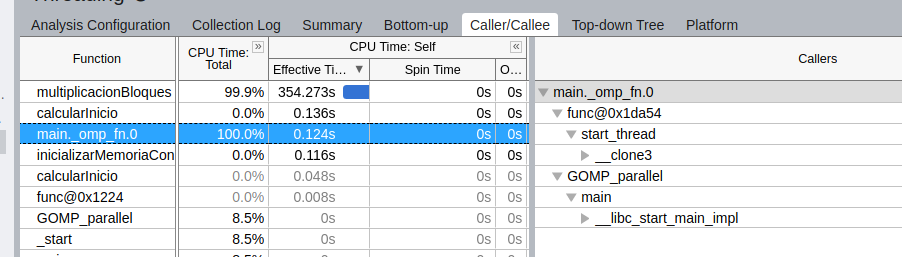
\includegraphics[scale=0.42]{./images/vtuneompTabla.png}
    \centering
    \caption{ Ventana {\it Caller/Callee} de la aplicación Intel VTune donde podemos ver el tiempo que transcurre en CPU cada función, en este caso de la rutina {\it MMB} implementada con OpenMP.}
    \label{fig:vtune-tablaomp}
\end{figure}

Para Intel TBB, tenemos la Imagen~\ref{fig:vtune-tablatbb}, donde se observa también la llamada a lo que sería el reparto de trabajo y la creación de los hilos. Esto es la llamada a {\it operator}. En el desglose a la derecha podemos ver también la llamada a {\it blocked\_range2d} (vista en la implementación de Intel TBB). En este último método transcurren 0,244 segundos. Dicho esto, se puede ver que la diferencia de tiempos que hemos visto a favor de Intel TBB en el Apartado~\ref{section:ompvstbb} no se debe a la rapidez en crear hilos y la asignación de trabajo, pues Intel TBB tarda más, aunque es un tiempo que se diluye en la ejecución de forma que finalmente no se aprecia mucho. Pero entonces, ¿dónde puede ser que OpenMP vaya más lento que Intel TBB según los tiempos de la tabla~\ref{tab:eje_mem}?. Pues bien, en la herramienta Intel VTune también podemos observar que la función {\it multiplicacionBloques} es más lenta en OpenMP que en Intel TBB, y esto se puede deber, en gran parte, a que en OpenMP se hace la asignación de trabajo una sola vez y se ejecutan todos los hilos a la vez, haciendo que estos accedan a regiones de memoria lejanas entre sí y haciendo que los aciertos en caché y memoria principal disminuyan. En cambio, en Intel TBB se puede observar que el reparto no se hace solo de una vez (por eso quizás tarda un poco más la llamada de su librería). Es decir, un hilo en vez de recibir todo el trabajo de golpe, recibe una parte, y cuando termina se le asigna otra parte, de forma que empieza de nuevo los bucles paralelos. Esto hace que dos hilos o más puedan estar trabajando con regiones memorias muy cercanas entre sí, haciendo que haya más aciertos en caché que en OpenMP y, por tanto, el tiempo de {\it multiplicacionBloques} sea menor, y en global el de la ejecución del programa.


\begin{figure}[htbp]
    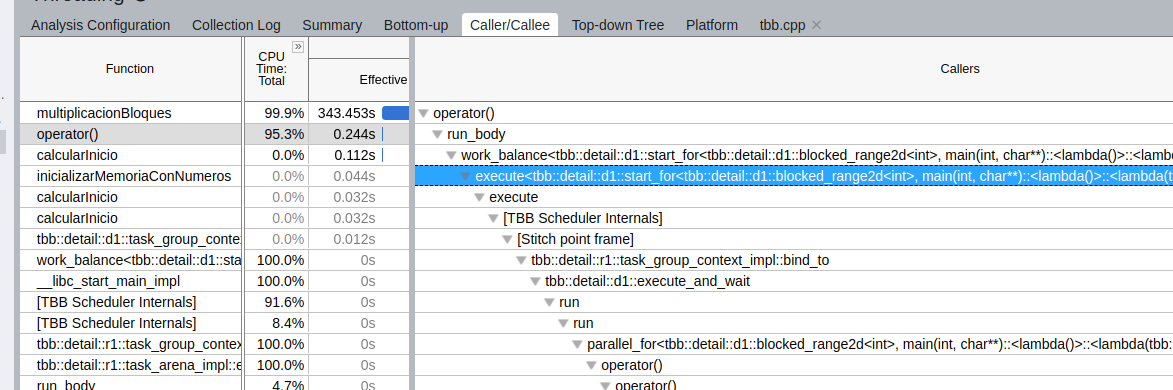
\includegraphics[scale=0.33]{./images/vtunetbbTabla.png}
    \centering
    \caption{ Ventana {\it Caller/Callee} de la aplicación Intel VTune donde podemos ver el tiempo que transcurre en CPU cada función, en este caso de la rutina {\it MMB} implementada con Intel TBB.}
    \label{fig:vtune-tablatbb}
\end{figure}

\subsubsection{Open MPI vs Intel MPI}
\label{sec:mpi-impi}
Para la comparación entre Open MPI e Intel MPI, mediante Intel VTune, vamos a usar matrices de 4096$\times$4096, un tamaño de bloque de 16$\times$16 (como se dijo en la configuración) y 4 procesadores, ya que es el máximo que tenemos disponible en el ordenador, pues solo disponemos de 6 nodos y tiene que ser potencia de 2 para que funcione correctamente la ejecución del programa en memoria distribuida.

La herramienta Intel VTune tiene varios apartados donde se puede ver información relevante de la ejecución del programa como dijimos, esta vez, no miraremos la eficiencia de la CPU, pues es irrelevante ya que en los dos casos se está utilizando desde el inicio hasta el final 4 procesos que transcurren paralelamente. Por ello, nos fijamos solo en {\it Caller/callee}, donde podemos seleccionar específicamente los tiempos de las llamadas a la librería que queremos. En este caso vamos a ver los tiempos de ejecución que han ocupado las distintas funciones de las librerías de Open MPI e Intel MPI, ya que es lo interesante de esta comparación.

En la Imagen~\ref{fig:vtune-mpi} se pueden ver los tiempos que transcurren en las llamadas a los métodos de la librería de Open MPI. En ella vemos que la llamadas más costosa es {\it MPI\_BARRIER}, la cual se puede obviar porque se usan al inicio para que empiecen todos los hilos a la vez. La siguiente más costosa es la de {\it PMPI\_Gather}, que corresponde a la función {\it MPI\_Gather} de la librería Open MPI, con la que todos los procesos reunían el resultado de su trabajo en el proceso principal (proceso 0). 
\begin{figure}[htbp]
    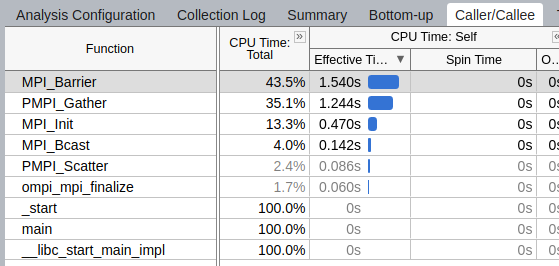
\includegraphics[scale=0.6]{./images/vtunempiTabla.png}
    \centering
    \caption{Ventana {\it Caller/Callee} de la aplicación Intel VTune donde podemos ver el tiempo que transcurre al usar las funciones de la librería Open MPI en la ejecución de la rutina {\it MMB} con la versión de Open MPI.}
    \label{fig:vtune-mpi}
\end{figure}

Para el análisis de Intel MPI tenemos la Imagen~\ref{fig:vtune-impi}, donde podemos observar de nuevo los tiempos que transcurren, esta vez aunque con los mismos nombres, en las funciones de la librería de Intel MPI. Como vemos, los tiempos en todas las distintas llamadas son considerablemente menores que en Open MPI, pero estas diferencias solo ocurren una vez en la ejecución, lo que hace que se diluyan en el tiempo de ejecución del programa y no se vean claramente como se demuestra en el Apartado~\ref{section:mpivsimpi}. Visto esto, podemos decir con Intel VTune que las llamadas a la librería de Intel MPI son menos costosas que las de Open MPI, y que en un programa donde se realizan muchas más comunicaciones (pasos de mensajes) entre los procesos es posible que la  diferencia de tiempo fuese más reseñable que la que se encuentra usando la rutina {\it MMB}.

\begin{figure}[htbp]
    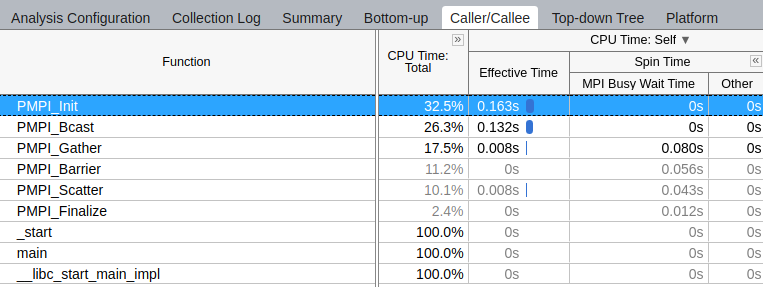
\includegraphics[scale=0.5]{./images/vtuneimpiTabla.png}
    \centering
    \caption{Ventana {\it Caller/Callee} de la aplicación Intel VTune donde podemos ver el tiempo que transcurre al usar las funciones de la librería Intel MPI en la ejecución de la rutina {\it MMB} con la versión de Intel MPI.}
    \label{fig:vtune-impi}
\end{figure}

\subsubsection{Versión híbrida de Open vs versión híbrida de Intel}
Para esta última comparativa en Intel VTune, hemos usado matrices de 4096$\times$4096, un tamaño de bloque de 16$\times$16, 4 procesadores y 3 hilos por cada procesador. De esta forma, conseguimos utilizar todas las prestaciones que nos da el computador.

Mediante Intel VTune, hemos visto una idea de por qué en los tiempos de la Tabla~\ref{tab:eje_hib}, los tiempos de ejecución del híbrido de Intel eran considerablemente menores que los del híbrido de Open, aunque recordemos que esta comparación es en el ordenador del alumno y no en el clúster como son los tiempos de las tablas. Siguiendo con ello, en la Imagen~\ref{fig:vtune-hibmpi}, se observa para el híbrido de Open, que el coste de las llamadas a las funciones de la librería Open MPI es más costoso respecto al que se muestra en la Imagen~\ref{fig:vtune-mpi}, que es cuando se usaba sola la versión de Open MPI, destacando que en las dos implementaciones se han usado 4 procesos. En cuanto al híbrido de Intel, el coste de estas llamadas se sigue manteniendo respecto al de Intel MPI, viéndose en la Imagen~\ref{fig:vtune-ihibmpi} el del híbrido y en la Imagen~\ref{fig:vtune-impi} el de Intel MPI solo.

\begin{figure}[htbp]
    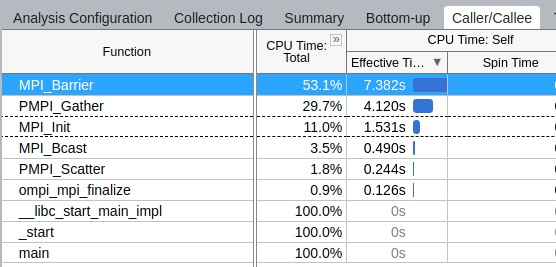
\includegraphics[scale=0.7]{./images/vtunehibmpi.png}
    \centering
    \caption{ Ventana {\it Caller/Callee} de la aplicación Intel VTune donde podemos ver el tiempo que transcurre al usar las funciones de la librería Open MPI en la ejecución de la rutina {\it MMB} con la versión híbrida de Open.}
    \label{fig:vtune-hibmpi}
\end{figure}

\begin{figure}[htbp]
    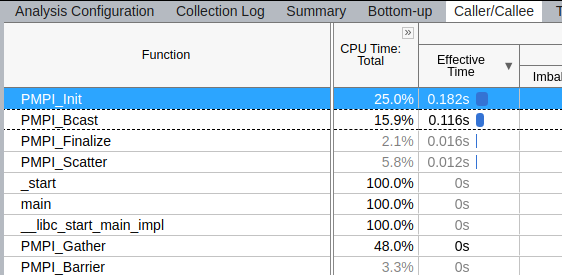
\includegraphics[scale=0.7]{./images/vtuneihibimpi.png}
    \centering
    \caption{Ventana {\it Caller/Callee} de la aplicación Intel VTune donde podemos ver el tiempo que transcurre al usar las funciones de la librería Intel MPI en la ejecución de la rutina {\it MMB} con la versión híbrida de Intel.}
    \label{fig:vtune-ihibmpi}
\end{figure}

Luego, para el híbrido de Open, se puede ver que, en la Imagen~\ref{fig:vtune-hibomp}, los tiempos de la función de {\it multiplicacionBloques} se ha disparado en cuanto al de la Imagen~\ref{fig:vtune-tablaomp}, cuando se usa OpenMP solo. 


Debido a esto, es posible que los costes de la llamada a las funciones de Open MPI se hayan visto incrementados. Esta subida de tiempo ocurre sobretodo con {\it MPI\_Gather}, porque se ejecuta al final de la rutina {\it MMB} para reunir el trabajo entre los procesos y es posible que otro proceso haya tenido muchos más fallos de caché que los otros, haciendo que este se descuelgue y sea más lento, resultando en que si el proceso 0 ha terminado antes se quede en espera creciendo el tiempo de {\it MPI\_Gather}. 

\begin{figure}[htbp]
    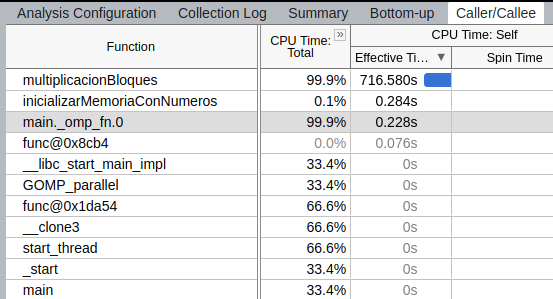
\includegraphics[scale=0.7]{./images/vtunehibomp.png}
    \centering
    \caption{Ventana {\it Caller/Callee} de la aplicación Intel VTune donde podemos ver el tiempo que transcurre en CPU cada función, en este caso de la rutina {\it MMB} implementada con el híbrido de Open.}
    \label{fig:vtune-hibomp}
\end{figure}

En resultado, en el ordenador del alumno, es posible que los problemas que tiene OpenMP en cuanto a los accesos de caché, los traslade también a Open MPI, de forma que el híbrido de Open se entorpezca en gran medida y quedando por detrás que el híbrido de Intel.

\newpage
%%%%%%%%%%%%%%%%%%%%%%%%%%%%%%%%%%%%%%%%%%%%%%%%%%%%%%%%%%%%%%%%%%%%%%%%%%%%%%%
\section{Conclusiones y Trabajo Futuro} \label{sec:conclusiones}
%%%%%%%%%%%%%%%%%%%%%%%%%%%%%%%%%%%%%%%%%%%%%%%%%%%%%%%%%%%%%%%%%%%%%%%%%%%%%%%

\subsection{Conclusiones}
El principal objetivo de este trabajo era realizar una comparativa entre las librerías de OpenMP e IntelTBB en memoria compartida, Open MPI e Intel MPI en memoria distribuida (paso de mensajes) y entre los híbridos de Open e Intel.

Como primera conclusión que hemos obtenido podemos decir que, aunque OpenMP es más sencillo de implementar, también es más lento que Intel TBB. Esta última librería internamente funciona mejor que OpenMP y, además, nos permite realizar también muchísimas otras posibilidades. Aunque en nuestra rutina {\it MMB} solo hemos podido paralelizar los bucles, donde Intel TBB ha destacado sobre OpenMP, porque internamente reparte de forma distinta el trabajo a sus hilos de forma que hace que aumente los aciertos en caché y, por ello, disminuya el tiempo de ejecución respecto a OpenMP.

Entre Open MPI e Intel MPI se ha visto que los tiempos de ejecución promedios son muy similares y que apenas podemos apreciar diferencias. La herramienta Intel VTune nos muestra que las llamadas a las funciones de comunicación de la librería de Open MPI son ligeramente más costosas que en Intel MPI. Esto nos hace decantarnos a que, para nuestra rutina {\it MMB} y nuestros entornos de ejecución (nodo Venus del clúster de la Facultad de Informática y ordenador personal del alumno), Intel MPI sea ligeramente mejor opción que Open MPI. 

Con el híbrido de Open los resultados no han sido los esperados teóricamente, y es que, tanto con el ordenador del alumno, como en el nodo Venus, parece que se entorpecen cuando se juntan las librerías de OpenMP junto a la de  Open MPI para algunos tamaños de problema concretos. En cambio, el híbrido de Intel, para todos los tamaños, obtiene unos tiempos razonables viendo que la integración de Intel TBB con Intel MPI funciona bien. Igualmente, incluso cuando el híbrido de Open ha sacado los tiempos que se esperaban, el híbrido de Intel lo ha seguido superando debido a que las ventajas que tienen Intel TBB e Intel MPI respecto a OpenMP y Open MPI se han mantenido cuando se han implementado los híbridos e incluso éstas han aumentado haciendo que el híbrido de Intel destaque sobre el de OpenMP.

Finalmente, el análisis de todas estas comparaciones se ha hecho centrándonos principalmente en los tiempos de ejecución que han dado las distintas implementaciones y, gracias al uso de la herramienta Intel VTune también hemos podido explicar el motivo de los distintos tiempos de ejecución, y así, hemos podido realizar una comparación y un análisis más profundo entre las distintas librerías de Open e Intel.



\subsection{Trabajo Futuro}
En este trabajo se ha desarrollado la rutina para la multiplicación de matrices por bloques ({\it MMB}) con la que hemos podido realizar una comparación entre las librerías de Open e Intel orientadas a las programación paralela. Aunque, se han obtenido unas conclusiones sobre estas librerías, éstas no son definitivas pues se podrían realizar otras comparaciones y análisis más profundos. Por tanto, para finalizar esta memoria se presentan algunas vías futuras a explorar para analizar en profundidad estas librerías como son:

\begin{itemize}
    \item Para la comparación entre Open MPI e Intel MPI, implementar una rutina en la que se tenga que realizar uso de las distintas llamadas de estas librerías y, además, que estas llamadas se tengan que realizar varias veces durante la ejecución de la rutina, dando así lugar a que se puedan ver claramente, las diferencias que hay entre usar los métodos de una librería u otra, y las ganancias que hay en una respecto a la otra librería.
    \item Igual que con MPI, se puede coger las librerías de OpenMP e Intel TBB y crear otra rutina que no se paralelize mediante bucles, y donde el efecto de los aciertos y fallos de la caché no sean tan relevante. Por ejemplo, una rutina que funcione mediante tareas, viendo en profundidad cómo se comportan estas dos librerías con esta implementación, obteniendo así, otras conclusiones sobre el uso de estas dos librerías.
    \item Finalmente, se puede realizar una comparativa cuando se utiliza una programación multi-plataforma (como OpenACC~\cite{openACC}) de las prestaciones obtenidas con respecto a usar OpenMP+OpenMPI e IntelTBB+IntelMPI.
\end{itemize}

\newpage

%%%%%%%%%%%%%%%%%%%%%%%%%%%%%%%%%%%%%%%%%%%%%%%%%%%%%%%%%%%%%%%%%%%%%%%%%%%%%%%
\section{Bibliografía} \label{sec:bibliografia}
%%%%%%%%%%%%%%%%%%%%%%%%%%%%%%%%%%%%%%%%%%%%%%%%%%%%%%%%%%%%%%%%%%%%%%%%%%%%%%%

\begin{thebibliography}{}

\bibitem{openACC}
OpenACC: \url{https://www.openacc.org/}

\bibitem{vtune}
Intel VTune Profiler: \url{https://software.intel.com/content/www/us/en/develop/tools/oneapi/components/vtune-profiler.html#gs.cm3p8h}

\bibitem{tbb}
Intel Threading Building Blocks: \url{https://software.intel.com/content/www/us/en/develop/tools/oneapi/components/onetbb.html#gs.cm3pi7}

\bibitem{impi}
Intel MPI: \url{https://software.intel.com/content/www/us/en/develop/tools/oneapi/components/mpi-library.html#gs.cm8q86}

\bibitem{who}
The OpenMP API specification for parallel programming. Who’s Using OpenMP?:
\url{https://www.openmp.org/about/whos-using-openmp/}

\bibitem{macros}
DATADVANCE’s MACROS. Build, explore, optimize and deploy industrial Digital Twins at scale across various industries: \url{https://www.datadvance.net}

\bibitem{altair}
Altair RADIOSS. Product Performance Under Dynamic Loadings:
\url{https://www.altair.com/radioss}

\bibitem{super1}
IBM RoadRunner: \url{https://www.techtarget.com/searchdatacenter/definition/IBM-Roadrunner}

\bibitem{super2}
Shida, Naoyuki Sumimoto, Shinji Uno, Atsuya. (2012). MPI Library and Low-Level Communication on the K computer. Fujitsu scientific \& technical journal. 48. 324-330.

\bibitem{moose}
GitHub de la aplicación {\it MOOSE}: \url{https://github.com/idaholab/moose}

\bibitem{madness}
Github de la aplicación {\it MADNESS}: \url{https://github.com/m-a-d-n-e-s-s/madness}

\bibitem{super3}
Ohio Supercomputer Center. An OH-TECH Consortium Member: \url{https://www.osc.edu/resources/available_software/software_list/intel_mpi}

\bibitem{LeyMoore}
Moore, G. (1965). Moore’s law. Electronics Magazine, 38(8), 114.

\bibitem{Amdahl}
Amdahl, G. M. (2013). Computer architecture and Amdahl's law. Computer, 46(12), 38-46.

\bibitem{endMoore}
The End of Moore’s Law in Detail and Starting a New Golden Age: \url{https://www.nextbigfuture.com/2019/02/the-end-of-moores-law-in-detail-and-starting-a-new-golden-age.html}

\bibitem{genasis}
GenASiS. General Astrophysical Simulation System: \url{http://genasis.xyz/}

\bibitem{riverflo2d}
Hydronia LLC. Hydraulic Modeling Specialists. Developers and Distributors of RiverFlow2D and OilFlow2D: \url{http://www.hydronia.com/}


\bibitem{Bukhamsin}
Ahmed Bukhamsin, Mohamad Sindi, and Jallal Al-Jallal. 2010. Using the Intel MPI benchmarks (IMB) to evaluate MPI implementations on an Infiniband Nehalem Linux cluster. In Proceedings of the 2010 Spring Simulation Multiconference (SpringSim '10). Society for Computer Simulation International, San Diego, CA, USA, Article 240, 1–4. \url{https://doi.org/10.1145/1878537.1878787}

\bibitem{openmp}
OpenMP. The OpenMP API specification for parallel programming:
\url{https://www.openmp.org/}

\bibitem{openmpi}
Open MPI. Open Source High Performance Computing: 
\url{https://www.open-mpi.org/}

\bibitem{icmat}
Instituto de ciencias matemáticas. Introducción a la programación paralela y computación en clúster: 
\url{https://www.icmat.es/downloads/computing/hpc-parallel-programming-intro.pdf}

\end{thebibliography}

\newpage

%%%%%%%%%%%%%%%%%%%%%%%%%%%%%%%%%%%%%%%%%%%%%%%%%%%%%%%%%%%%%%%%%%%%%%%%%%%%%%%%
\appendix

\section{Versión Paralela con Intel TBB} \label{app:A}
\lstset{language=C++,
                keywordstyle=\color{blue},
                stringstyle=\color{red},
                commentstyle=\color{red},
                morecomment=[l][\color{magenta}]{\#}
}
\begin{lstlisting}
#include <tbb/parallel_for.h>
#include <tbb/blocked_range2d.h>
#include <tbb/task_arena.h>
 ...
 int main(int argc, char* argv[]){
 ...
//Matrices multiplicadoras y resultado
int* matA, matB, matRes;
int filas,columnas;
//Tamano de submatrices NxN
int tam;
//Num. submatrices a lo largo y ancho al dividir 
//por el tamano de las submatrices
int numMatFil = filas/tam;
int numMatCol = columnas/tam;
//Limitamos los hilos en TBB
tbb::task_arena limited(numHilosTBB); 
//Ejecutamos el codigo paralelo de TBB
limited.execute([&]{
    tbb::parallel_for(tbb::blocked_range2d<int>
    (0, numMatFil, 0,numMatCol),
    [&](const tbb::blocked_range2d<int> r) {
        for (int i = 0; i < numMatFil;i++) {
            for (int j = 0; j < numMatCol;j++) { {
                for (int k = 0; k < numMatFil;k++) {
                    //Num. de submatriz que se 
                    //multiplica en la llamada
                    int numMatRes = i * numMatFil + j;
                    int numMatA = (i * numMatFil) + k;
                    int numMatB= j + (k * numMatFil);
                    //Realizamos la multiplicacion
                    multPorBlo(matA,matB,matRes,...);
                }
            }
        }
    });
});//Fin codigo paralelo
 ...
 return 0;
}

\end{lstlisting}


\newpage
\section{Versión Paralela con Intel MPI} \label{app:B}
\lstset{language=C++,
                keywordstyle=\color{blue},
                stringstyle=\color{red},
                commentstyle=\color{red},
                morecomment=[l][\color{magenta}]{\#}
}
\begin{lstlisting}
#include <mpi.h>
 ...
int main(int argc, char* argv[]){
 //Desde aqui se pueden realizar llamadas a MPI
 MPI_Init(&argc, &argv);
 ...
//La matriz B sera una matriz que tienen todos
//aunque cada uno en su memoria correspondiente
int* matB;
int filas,columnas;
//Se calcula el trabajo que tendra cada uno
int filas_local = filasA / numTrabajadores;
int columnas_local = columnasA;
//Estas dos matrices, seran la parte de trabajo
//que tiene cada trabajador y a la vez su resultado
int* matA_loc = malloc(...);
int* matRes_loc = malloc(...);


//Envia la informacion el trabajador principal
if (procesador_principal) {
    //Inicializamos individualmente la matriz B
    matB = inicializar(filas, columnas);
    //La matriz B la tienen entera todos los hilos
    //Repartimos la matriz B con los otros trabajadores
    int tamMatEnviado = filas * columnas;
    MPI_Bcast(matB, tamMatEnviado, MPI_INT, ...);

    //Inicializamos individualmente la matriz A
    matA = inicializar(filas, columnas);
    //Dividimos la matrizA en cada trozo que toca
    //La matriz A no la utiliza entera cada trabajador
    int* matA = inicializar(filas, columnas);
    //Dividimos la matrizA y se lo enviamos a cada
    //trabajador a su respectiva matriz(matA_loc)
    int tamMatEnviado = filas_local * columnas_local;
    MPI_Scatter(matA, tamMatEnviado, MPI_INT, matA_loc, ...);
    //Liberamos la matriz A que ya nadie va a usar
    free(matA);
}
else {//Ahora reciben la informacion los trabajadores
    //La matriz B la tienen entera todos los hilos
    int tamMatRec = filas * columnas;
    matB = malloc(...);
    MPI_Bcast(..., matB, tamMatRec, MPI_INT, ...);
    //Recibimos el trozo de la matrizA que nos corresponde
    int tamMatRec = filas_local * columnas_local;
    MPI_Scatter(..., matA_loc, tamMatRec, MPI_INT, ...);
}
 ...
//Realizariamos la multiplicacion por bloque
//secuencialmente cada trabajador
 multBloqSecuencial(matA_loc,matB,matRes_loc);
 ...
//Ahora tenemos que juntar los resultados de los distintos
//trabajadores enviandoselo todo al trabajador principal
if (procesador_principal){
    //Creamos la matriz en la que recibimos los resultados
    int* matrizTotal = malloc();
    MPI_Gather(matRes_loc, .., matrizTotal, .., 0, ..);
    //Escribimos matriz resultado o lo que hiciera falta
    ...
    //Luego liberamos
    free(matrizTotal);
}else{
    //El 0 indica el trabajador al que se le envia
    //Y el NULL se refiere a que este trabajador no recibe
    //ningun dato, ya que no tiene el id igual a 0
    MPI_Gather(matRes_loc, .., NULL, .., 0, ..);
}

//Liberariamos memoria de cada procesador reservada
...
MPI_Finalize();
 ...
 return 0;
}
\end{lstlisting}
%%%%%%%%%%%%%%%%%%%%%%%%%%%%%%%%%%%%%%%%%%%%%%%%%%%%%%%%%%%%%%%%%%%%%%%%%%%%%%%%

\end{document}
